%!TEX TS-program = xelatex
%!TEX encoding = UTF-8 Unicode

\documentclass{Dissertate}

\newcommand{\species}[1]{\textit{#1}}
\newcommand{\todo}[1]{{\color{red}{TODO: #1}}}
\newcommand{\p}[1]{#1~\%}
\newcommand{\eg}{\textit{e.g.}}
\newcommand{\ie}{\textit{i.e.}}

\begin{document}

% the front matter:
% title page, license page, abstract page,
% tables of contents, figures, and tables
% dedication, acknowledgements

% make sure you personalize frontmatter/personalize.tex
\frontmatter

% line spacing
\setstretch{\dnormalspacing}

% include each chapter...
\setcounter{chapter}{0}  % start chapter numbering at 0
%!TEX root = ../dissertation.tex
\chapter{Introduction}
\label{introduction}

\newthought{We are currently experiencing a mass extinction event} that parallels
other episodes in earth's history with high rates of biodiversity
decline \citep{Pimm1995, Dirzo2003, Schipper2008, Barnosky2011,
Dirzo2014}. Other than the five previous major extinction events
\citep{Kolbert2014}, it is anthropogenic in origin \citep{Leakey1996,
Ceballos2015} and is associated with global warming \citep{Cook2016,
Wuebbles2017}, large-scale deforestation \citep{Wright2005}, destruction
of marine and freshwater habitats \citep{Burkhead2012}, and introduction
of invasive species \citep{Mooney2001}, all hallmarks of human
influence. Put shortly, the rate at which species go extinct is alarming
\citep{Newbold2016, Ceballos2017, Hallmann2017}, and our children will
likely experience a world with less than half the biodiversity we know
today. While this issue has raised the attention of country leaders and
conservation policies are being put in place worldwide
\citep{Puntaru2017}, this might not be enough to reverse the trend
without sustaining irreparable damage to the ecosystems of the planet.
To make matters worse, there are signs that the issue, despite its
urgency, is fading from public awareness \citep{Kusmanoff2017}. 

Conservation efforts require intimate knowledge of the systems they aim
to preserve: Of course, we cannot save what we do not know. The road
towards understanding the biology and the interaction of species is,
however, travelled on multiple levels. It is not enough to observe the
behaviour or the feeding preferences of an animal to understand the
impact of it being removed from its habitat. It is also not enough to
describe functional morphology to gain insight on ecological
implications. Neither is it sufficient to analyze the genes and draw
conclusions based on their composition and structure. Profound
understanding of any system can only be gained by studying it from
multiple angles and with interdisciplinary approaches. One such approach
is to sequence and analyze the genome of a species: the ``source code of
life'' that defines, by a manifold of means, its appearance, features,
behaviour and interactions with the environment.

The genome, that is, the entirety of DNA of an organism is a composition
of different functional complexes. It does not only contain genes, which
are transcribed to messenger RNA and translated into the proteins that
make up cells and, ultimately, all organisms; in fact, the human gene
repertoire of around 23,000 genes makes up only around \p{2} of the human
genome \citep{Makalowski2001} (Figure \ref{fig:human-genome}). More
prominent components of the human genome include introns (non-coding
sections of genes, around \p{26}), but by far the most voluminous chunk
consists of repetitive elements: DNA segments that occur in sometimes
many copies throughout the genome.  More than half of the three billion
base pairs (Gbp) of the human genome (\p{52}) is occupied by repetitive
elements \citep{Lander2001}. The major part of these repetitive elements
in the human genome, also called repeats, is formed by transposable
elements (\p{45} of the genome).

\begin{figure}
	\centering
  \begin{minipage}[c]{0.3\textwidth}
		\caption[Composition of the human genome]{Composition of the human
		genome. Almost half of the three billion base pairs in the genome is
		attributed to transposable elements of various classes (DNA transposons,
		LTR retrotransposons, LINEs, SINEs). Data source: \citet{Lander2001}}
		\label{fig:human-genome}
  \end{minipage}\hspace{3em}
  \begin{minipage}[c]{0.3\textwidth}
		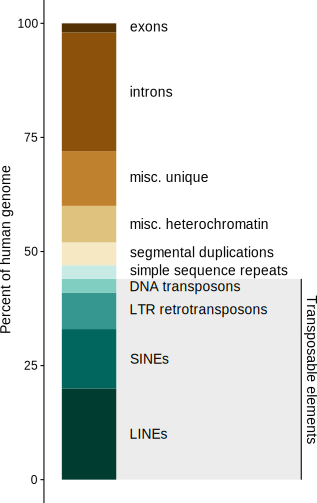
\includegraphics[width=\textwidth]{human}
  \end{minipage}
\end{figure}

Transposable elements (TEs) are also known as ``jumping genes'' or
``parasitic DNA''. They were discovered in the 1940s by their defining
property, the capability of movement within the genome
\citep{McClintock1950}. By duplicating themselves through various
mechanisms that depend on the TE type, TEs can reach copy numbers in the
thousands \citep{Petersen2018} and, like in the human genome (Figure
\ref{fig:human-genome}), be a major contributor to the genome size. This
genome ``inflation'' effect due to TE proliferation has been observed
throughout eukaryotes in general \citep{Chenais2012}, and reiterated in
vertebrates \citep{Chalopin2015}, arthropods \citep{Petersen2018}, and
plants \citep{Staton2015}. 

The genomes of mammals, such as human, and birds exhibit much less
variation in size than, for example, the genomes of arthropods or
amphibians \citep{Gregory2005}. In mammals, genome size varies around
five-fold and in birds even only around two-fold, whereas in insects,
the spread is around 240-fold (Figure \ref{fig:genome-size-spread},
Table \ref{tab:genome-size-spread} on page
\pageref{tab:genome-size-spread}). This immense variation surpasses that
of amphibians, where some species have huge genomes of up to 118 Gbp,
and is paralleled only by the group of bony fishes (Osteichthyes,
excluding lungfishes), which exhibit a genome size spread of around
220-fold. Before the discovery of TEs and non-coding DNA, such as
introns, in the genome, it was assumed that genome size should correlate
with perceived organismic complexity, but the fact that amoeba have
genomes with up to a staggering 670 Gbp \citep{Parfrey2008} did not fit
well with that assumption. This apparent contradiction was named the
``C-value paradox'' and later renamed to ``C-value enigma''
\citep{Gregory2007}, as still a connection between genome size and
organismic complexity appears absent.

\begin{figure}
\centering

\includegraphics[width=0.7\textwidth]{genome-size-spread}
\caption[Genome size spread in eukaryotes and prokaryotes]{Genome size
spread in eukaryotes and prokaryotes. The C-value is the amount of
haploid nuclear DNA in picogram (pg); one pg DNA is approximately 978
Mbp. Colors are ordered for chordate animals, invertebrate animals,
plants, fungi and algae, and prokaryotes.  Figure modified from
\citet{Gregory2004}.}
\label{fig:genome-size-spread}
\end{figure}

No matter the size, the genome needs to be maintained: repair mechanisms
and transcription machinery as well as error correction use energy. The
transcription and translation error rate increases with genome size
\citep{Zaher2009}, making more repairs necessary. Larger genome size has
been linked to decreased development rate \citep{White2000} and
increased oxygen requirements \citep{Vinogradov1997, Gregory2002}. In
plants \citep{Grime1983}, invertebrates \citep{Gregory2005}, and
vertebrates \citep{Horner1983, Olmo1982, Gregory2000}, it has been shown
that cell size increases with genome size \citep{Dufresne2011}. Larger
cells are also less efficient to maintain and proliferate, and they
divide more slowly \citep{Bennett1977}. In summary, a large genome comes
with a cost. What would be the benefit of having a large genome?

The more genetic material in the genome, the higher the likelihood of
random mutations \citep{Wielgoss2011}. Mutations provide the basis for
genotypic evolution: through natural selection, deleterious changes to
the genome will be removed from populations over time, and beneficial
changes --- or innovations --- prevail. A higher mutation rate is not
always a negative property: it also brings with it a higher rate of
beneficial mutations. Therefore, the genome is thought to reach an
equilibrium between the incurred metabolic cost of sustaining a high
mutation rate (\emph{i.e.}, the damage caused by deleterious mutations),
and the cost of mechanisms that reduce the mutation rate
\citep{Bernstein1987, Altenberg2011}.

The presence and activity of TEs can have disruptive influence on the
genome architecture. By inserting at critical positions, TEs can disable
genes \citep{Kazazian1988}. An insertion in regulatory sequence can
change gene expression \citep{Warnefors2010}. TEs, by way of their
repetitive nature, provide hotspots for ectopic (non-homologous)
recombination \citep{Lim1988, Gray2000, Fiston-Lavier2007}, thus
increasing the likelihood for segmental duplications, deletions, and
inversions \citep{Mathiopoulos1998, Remnant2013}. On the one hand, TEs
are obviously a source of potentially deleterious mutations. On the
other hand, TEs can be ``domesticated'' and genes exapted from TE
sequence \citep{Gahan2001, Daborn2002, Aminetzach2005, Chen2007},
inferring novel functions to the host. Such innovations can happen
within a few hundred generations \citep{Dolgin2006, Struchiner2009,
Kofler2015}. As a famous example, the melanism in the British peppered
moth --- which evolved camouflage matching the birch trees blackened as
a result of industrialisation --- is caused by TEs \citep{Hof2016}.
These observations document that TE activity can also have beneficial
effects on the host genome (especially in times of stress\todo{cite}),
and should therefore not be entirely subdued.

To keep the TE population in check, defenses that remove or silence TEs
have developed in host organisms. In many groups of organisms, a
multi-layered network of epigenetic regulation mechanisms evolved in
place to prevent TE activity at both the pre- and post-transcriptional
stage. In plants, an epigenetic modification called DNA methylation
prevents TEs from being transcribed and thus from transposing
\citep{Slotkin2007, Lisch2009}. After transcription, proteins from the
RNA interference (RNAi) pathway can disable messenger RNA and thereby
silence TEs \citep{Buchon2006}. Similarly, a class of non-coding RNA,
so-called Piwi-interacting RNA (piRNA) protect the integrity of the
genome, in particular in germline cells, by forming a complex with Piwi
proteins, which can bind and cleave RNA \citep{Zeng2011}. This complex
can recognize and silence target TEs in the RNA stage \citep{Siomi2011, Mondal2018}.
Similar systems were identified in vertebrate genomes \citep{Suzuki2008,
Schubeler2015}; DNA methylation is thought to be a genome defense
mechanism in mammals as well \citep{Yoder1997}. Interestingly,
vertebrate genomes are globally methylated, and in plant genomes, only
gene bodies and TEs are methylated \citep{Suzuki2008}. Fungal genome
exhibit an even more mosaic-like methylation pattern: here, only TEs are
methylated and genes are not. In invertebrates, TEs tend to be
unmethylated; the fruit fly \species{Drosophila melanogaster} does not
even have the methyltransferase enzyme. Likewise, some butterfly species
have lost RNAi pathway genes \citep{Pauli2016}. Thus, these genome
defenses appear to be modular and complementary to one another. They are
effective to a certain extent: permanently inactive TEs become genetic
``cruft'' and are degraded by genetic drift (random mutations over time)
like other parts of the genome that are not subject to selection
\citep{Szitenberg2016}. As a result of these extensive silencing
techniques, it is not surprising that most of the TE population in
extant genomes is inactive \citep{Yoder1997, Zilberman2007}.

There are two major models to explain TE population dynamics in the
genome: the equilibrium model and the burst model \citep{Petrov2011,
Kofler2012, Cridland2013, Blumenstiel2014}. In the equilibrium model,
the TE insertion rate is assumed to be more or less constant, and TEs
are silenced and removed by purifying selection at a likewise constant
rate \citep{Charlesworth1983}. This way, insertion rate and
removal/silencing rate would cancel each other out, and the genome size
remains stable.  The equilibrium model provides a better fit for TE
dynamics under the effects of purifying selection \citep{Barron2014}
than the transposition burst model. The burst model, which is also
termed the non-equilibrium model, predicts that TEs undergo periods of
high transposition activity while otherwise proliferating at a constant
but lower rate. Under the transposition burst model, a positive
correlation between the TE age and frequency would be expected, which
better explains the observed TE age distribution in insect genomes as
well as the large genome size fluctuations during insect evolution,
given that TE abundance is a predictor for genome size
\citep{Alfsnes2017, Petersen2018a}.

Insects are among the most speciose groups of organisms on earth (Figure
\ref{fig:biodiversity}) and, since their appearance approximately 480
million years ago (Mya) \citep{Misof2014}, have conquered land,
freshwater, and air (but not saltwater). Protected by their hard
exoskeleton, insect representatives have invaded virtually all
conceivable ecosystems including human habitations \citep{Bertone2016}.
Insects are immensely diverse in morphology \citep{Grimaldi2005} and
often highly specialized towards a specific food source, habitat, or
lifestyle. Bees, wasps, ants, and termites, for example, form eusocial
communities with a complex caste system. As disease vectors, mosquitoes
are responsible for more human deaths than all other animals combined
\citep{WHO2017, Linnell2011, Lamarque2009, DeMaddalena2008,
Kasturiratne2008, Packer2005}. Beetles and grasshoppers are an important
source of food for livestock and humans alike as well as a pest with
high economic impact \citep{Oliveira2014}. Obviously, insects play
pivotal roles in most ecosystems of the planet. Insect population
diversity and abundance, however, is declining \citep{Vogel2017} as a
result of widespread human influence (see above), with disastrous
reverberations at all levels of the local food chains.  In order to
mount efficient conservation efforts, a thorough understanding of insect
biology is required.

Despite their mega-diversity and ecological importance, insects are
astonishingly understudied on the genomic level compared to other
animals: On 2018-07-06, there were 1115 published non-insect animal
genome sequences in the NCBI database \citep{OLeary2016} (about \p{0.3}
of the total non-insect species diversity; Figure
\ref{fig:biodiversity}) and 493 insect genomes (\p{0.065}; about five
times less genomes per species).  That number is growing by about 50
genomes per year, however at this rate, it will take more than 150 years
to even sequence the genomes of 10 of the insect biodiversity.
During this time, many species will have gone extinct --- as it stands,
our sequencing efforts are losing the race against man-made biodiversity
loss.  Ever-improving, massively parallel sequencing technologies that
appeared during the early 2000's \citep{Behjati2013} have accelerated
the pace and accuracy at which genomes can be sequenced, but it will not
be enough. Of many insect species, we will never be able to obtain the
genomic source code, and this will hamper our understanding of the roles
these species occupied in the interaction network of their habitats.

Comparative genomics studies --- that is, investigations comparing
genomic features of more than one species --- are not only limited by
the fact that for many species, there is no genomic sequence information
available.  Additionally, comparative analyses have to take the
evolutionary history of the species into consideration \todo{cite},
usually in the form of a phylogenetic tree that conveys information on
the species' relationships. Among the approaches to infer a phylogenetic
species tree, the most informed, because based on matrices with data
points numbering in the millions, is reconstruction from amino acid or
nucleotide sequences. Phylogenetic species tree reconstruction, however,
regardless the method, is no simple task and relies on sophisticated
methods on all stages of the analysis (\eg, \citep{Misof2014,
Peters2017, Johnson2018}). Perhaps most of all, selection of the
phylogenetic markers (the features that distinguish species and define
their level of relatedness) is paramount. Most modern genomic studies
use single-copy genes that are found in all (or almost all) species. The
implied assumption is that these genes share a common ancestry and are
related via speciation events, that is, they are \emph{orthologous} to
one another \citep{Koonin2005} and their phylogeny reflects the species
phylogeny.

Several commonly used methods to identify orthologous genes rely on
clustering nucleotide or amino acid sequences based on their similarity
\citep{Chen2007a}. Since orthologs tend to be more similar to each other
than to all other genes in the genomes under comparison
\citep{Altenhoff2012a}, the orthology hypothesis can be tested via a
bi-directional search applying a best reciprocal hit (BRH) criterion:
Only if the gene in question returns the best hit in both directions it
can be assumed to be orthologous. By clustering genes that share BRH
relations, one can form clusters of orthologous genes (COGs), or simply
orthologous groups (OGs) \citep{Altenhoff2012}. This approach has been
implemented in several software packages for use in genomic datasets
(\eg, \citep{Li2003, Tatusov2003, Berglund2008, Zdobnov2017}).


\begin{figure}
\centering
\includegraphics[width=0.7\textwidth]{number-of-species}
\caption[Biodiversity by numbers of species]
{Insects contribute more than half of the currently known species
diversity.}
\label{fig:biodiversity}
\end{figure}

\section{Roadmap}

Insects are mega-diverse but genomically understudied --- insect
phylogeny on family level mostly unresolved --- 1KITE attempts to change
that --- orthology prediction crucial part of phylogenetic analysis ---
Orthograph identifies orthologs in transcriptomes --- Research questions
--- insect mobilome diversity and evolution --- dynamics of genome size
evolution in insects --- chapter 1: Mobilome --- chapter 2: Genome size
dynamics --- chapter 3: Orthograph --- papers using Orthograph are in
appendix

\begin{table}
\centering\footnotesize
\caption[Genome size spread in Metazoa]{Genome size spread in Metazoa.
Values are in picogram DNA; one pg is approx. 978 mega-basepairs (Mbp).
Data from the Genome Size Database \citep{Gregory2018},
\url{http://www.genomesize.com}, accessed 2018-05-07.}
\label{tab:genome-size-spread}
\begin{tabular}{@{}lllrrrr@{}}
\toprule
Phylum     & Subphylum   & Class          & n    & min  & max   & $\Delta$fold \\
\midrule
Annelida   & --          & Oligochaeta    & 35   & 0.43 & 7.64  & 17.77  \\
Annelida   & --          & Polychaeta     & 100  & 0.06 & 7.2   & 120    \\
Arthropoda & Chelicerata & Arachnida      & 148  & 0.08 & 7.5   & 93.75  \\
Arthropoda & Crustacea   & Branchiopoda   & 68   & 0.16 & 2.91  & 18.19  \\
Arthropoda & Crustacea   & Copepoda       & 73   & 0.14 & 14.68 & 104.86 \\
Arthropoda & Crustacea   & Malacostraca   & 241  & 0.68 & 64.62 & 95.03  \\
Arthropoda & Hexapoda    & Insecta        & 1353 & 0.07 & 16.93 & 241.86 \\
Chordata   & Vertebrata  & Amphibia       & 932  & 0.95 & 120.6 & 126.95 \\
Chordata   & Vertebrata  & Aves           & 903  & 0.91 & 2.16  & 2.37   \\
Chordata   & Vertebrata  & Chondrichthyes & 199  & 1.51 & 17.05 & 11.29  \\
Chordata   & Vertebrata  & Mammalia       & 816  & 1.63 & 8.4   & 5.15   \\
Chordata   & Vertebrata  & Osteichthyes   & 1909 & 0.34 & 74.86 & 220.18 \\
Chordata   & Vertebrata  & Reptilia       & 423  & 1.05 & 5.44  & 5.18   \\
Mollusca   & --          & Bivalvia       & 108  & 0.65 & 5.4   & 8.31   \\
Mollusca   & --          & Gastropoda     & 149  & 0.43 & 7.85  & 18.26  \\
Nematoda   & --          & Secernentea    & 72   & 0.02 & 2.5   & 125    \\
\bottomrule
\end{tabular}
\end{table}

%!TEX root = ../dissertation.tex
\begin{savequote}[75mm]
This chapter is intended for publication in BMC Evolutionary Biology.

Authors: Malte Petersen, David Armisén, Richard A. Gibbs, Lars Hering,
Abderrahman Khila, Georg Mayer, Stephen Richards, Oliver Niehuis, and
Bernhard Misof
%\qauthor{Firstname lastname}
\end{savequote}

\chapter{Diversity and evolution of the transposable element
repertoire in insects}
\label{cha:mobilome}

\section{Introduction}\label{introduction}

Repetitive elements, including transposable elements (TEs), are a major
sequence component of eukaryote genomes. In vertebrate genomes, for
example, the TE content varies from 6 \% in the pufferfish
\emph{Tetraodon nigroviridis} to more than 55 \% in the zebrafish
\emph{Danio rerio} \citep{Chalopin2015}. More than 45 \% of the human
genome \citep{deKoning2011} consist of TEs. In plants, TEs are even more
prevalent: up to 90 \% of the maize (\emph{Zea mays}) genome is covered
by TEs \citep{SanMiguel1996}. In insects, the genomic portion of TEs ranges
from as little as 1 \% in the antarctic midge \citep{Kelley2014} to as
large as 65 \% in the migratory locust \citep{Wang2014}.

TEs are known as ``jumping genes'' and traditionally viewed as selfish
parasitic nucleotide sequence elements propagating in genomes with
mainly deleterious or at least neutral effects on host fitness
\citep{Mackay_1989}. Due to their propagation in the genome, TEs are
thought to have a considerable influence on the evolution of the host's
genome architecture. By transposing into, for example, host genes or
regulatory sequences, TEs can disrupt coding sequences or gene
regulation, and/or provide hot spots for ectopic (non-homologous)
recombination that may induce chromosomal rearrangements in the host
genome such as deletions, duplications, inversions, and translocations
\citep{Burns2012}. For example, the shrinkage of the Y chromosome in the
fruit fly \emph{Drosophila melanogaster}, which consists mostly of TEs,
is thought to be caused by such intrachromosomal rearrangements induced
by ectopic recombination \citep{Adams2000}. As such potent agents for
mutation, TEs are also responsible for cancer and genetic diseases in
humans and other organisms
\citep{Vorechovsky2009,Chenais2015,Hancks2016}.

Despite the potential deleterious effects of their activity on gene
regulation, there is growing evidence that TEs can also be drivers of
genomic innovation generating selective advantages to the host
\citep{Casola2007,Gonzalez2008}. For example, it is well documented that
the frequent cleavage and rearrangement of DNA strands induced by TE
insertions provides a source of sequence variation to the host genome,
or that by a process called molecular domestication of TEs, host genomes
derive new functional genes and regulatory networks
\citep{Feschotte2008,Boehne2008,Santos_2014}.  Furthermore, many exons
have been \emph{de novo}-recruited from TE insertions in coding
sequences of the human genome \citep{Zhang2006}.  In insects, TE
insertions have played a pivotal role in the acquisition of insecticide
resistance \citep{Chen2007,Itokawa2010,Gahan2001}, as well as in the
rewiring of a regulatory network that provides dosage compensation
\citep{Ellison2013}, or the evolution of climate adaptation
\citep{Gonzalez2010,Kim2014}.



TEs are classified depending on their mode of transposition. Class I
TEs, also known as retrotransposons, transpose via an RNA-mediated
mechanism that can be circumscribed as ``copy-and-paste''. They are
further subdivided into long terminal repeat (LTR) retrotransposons and
non-LTR retrotransposons. Non-LTR retrotransposons include long and
short interspersed nuclear elements (LINEs and SINEs)
\citep{Malik1999,Eickbush2008}. Whereas LTR retrotransposons and LINEs
encode a reverse transcriptase, the non-autonomous SINEs rely on the
transcriptional machinery of autonomous elements, such as LINEs, for
mobility. Frequently found LTR retrotransposon families in eukaryote
genomes include Ty3/Gypsy, which was originally described in
\emph{Arabidopsis thaliana} \citep{Marin2000}, Ty1/Copia
\citep{Flavell1992}, as well as BEL/Pao \citep{de_la_Chaux2011}.

In Class II TEs, also termed DNA transposons, the transposition is
DNA-based and does not require an RNA intermediate. Autonomous DNA
transposons encode a transposase enzyme and move via a ``cut-and-paste''
mechanism. During replication, terminal inverted repeat (TIR)
transposons and Crypton-type elements cleave both DNA strands
\citep{Wicker2007}. Helitrons, also known as rolling-circle (RC)
transposons due to their characteristic mode of transposition
\citep{Kapitonov2001}, and Maverick elements \citep{Kapitonov2006}
cleave a single DNA strand in the process of replication. Class II also
encompasses non-autonomous DNA transposons such as miniature inverted
TEs (MITEs) \citep{Shirasawa2012}, which exploit and rely on the
transposase mechanisms of autonomous DNA transposons to replicate.

Previous reports on insect genomes describe the composition of TE
families in insect genomes as a mixture of metazoan and insect specific
TEs \citep{Feschotte2007}. Dedicated comparative analyses of TE
composition, however, have only been conducted on species of mosquitoes
\citep{Neafsey2014} and of drosophilid flies \citep{Sessegolo2016}.
Overall, surprisingly little effort has been put into characterizing TE
sequence families and TE compositions in insect genomes. While this lack
of knowledge is due to the low availability of sequenced insect genomes
in the past, efforts such as the i5k initiative \citep{Robinson2011}
have helped to increase the number of genome sequences from previously
unsampled insect taxa. With this denser sampling of insect genomic
diversity available, it now seems possible to comprehensively
investigate the TE diversity among major insect lineages.

Here, we present the first exhaustive analysis of the distribution of TE
classes in a sample representing half of the currently classified insect
orders and using standardized comparative methods implemented in
recently developed software packages.  Our results show similarities in
TE family diversity and abundance among the investigated insect genomes,
but also profound differences in TE activity even among closely related
species.

\section{Materials and methods}\label{materials-and-methods}

\subsection{Genomic data sets}\label{genomic-data-sets}

We downloaded genome assemblies of 42 arthropod species from NCBI
GenBank at \url{ftp.ncbi.nlm.nih.gov/genomes} (last accessed 2014-11-26;
supplementary table S2) as well as the genome assemblies of 31
additional species from the i5k FTP server at
\href{ftp://ftp.hgsc.bcm.edu:/I5K-pilot/}{ftp.hgsc.bcm.edu/I5K-pilot}
(last accessed 2016-07-08; supplementary table S2). Our taxon sampling
includes 21 dipterans, four lepidopterans, one trichopteran, five
coleopterans, one strepsipteran, 14 hymenopterans, one psocodean, six
hemipterans, one thysanopteran, one blattodean, one isopteran, one
orthopteran, one ephemeropteran, one odonate, one archaeognathan, and
one dipluran. As outgroups we included three crustaceans, one myriapod,
six chelicerates, and one onychophoran.

\subsection{Construction of species-specific repeat libraries and TE
annotation in the
genomes}\label{construction-of-species-specific-repeat-libraries-and-te-annotation-in-the-genomes}

We compiled species-specific TE libraries using automated annotation
methods. RepeatModeler Open-1.0.8 \citep{Smit2015} was employed to
cluster repetitive \emph{k}-mers in the assembled genomes and infer
consensus sequences. These consensus sequences were classified using a
reference-based similarity search in RepBase Update 20140131
\citep{Jurka2005}. The entries in the resulting repeat libraries were
then searched for using nucleotide BLAST in the NCBI nr database
(downloaded 2016-03-17 from
\href{ftp://ftp.ncbi.nlm.nih.gov/blast/db}{ftp.ncbi.nlm.nih.gov/blast/db})
to verify that the included consensus sequences are indeed TEs and not
annotation artifacts. Repeat sequences that were annotated as
``unknown'' and that resulted in a BLAST hit for known TE proteins such
as reverse transcriptase, transposase, integrase, or known TE domains
such as gag/pol/env, were kept and considered unknown TE nucleotide
sequences; but all other ``unknown'' sequences were not considered TE
sequences and therefore removed. The filter patterns are listed in
supplementary table S3. The filtered repeat library was combined with
the Metazoa-specific section of RepBase version 20140131 and
subsequently used with RepeatMasker 4.0.5 \citep{Smit2015} to annotate
TEs in the genome assemblies.

\subsection{Validation of Alu
presence}\label{validation-of-alu-presence}

To exemplarily validate our annotation, we selected the SINE Alu, which
was previously only identified in primates \citep{Kriegs2007}. We
retrieved a Hidden Markov model (HMM) profile for the AluJo subfamily
from the repeat database Dfam \citep{Hubley2016} and used the HMM to
search for Alu copies in the genome assemblies. We extracted the hit
nucleotide subsequences from the assemblies and inferred a multiple
nucleotide sequence alignment with the canonical Alu nucleotide sequence
from Repbase \citep{Jurka2005}.

\subsection{Genomic TE coverage and correlation with genome
size}\label{genomic-te-coverage-and-correlation-with-genome-size}

We used the tool ``one code to find them all'' \citep{Bailly-Bechet2014}
on the RepeatMasker output tables to calculate the genomic proportion of
annotated TEs. ``One code to find them all'' is able to merge entries
belonging to fragmented TE copies to produce a more accurate estimate of
the genomic TE content and especially the copy numbers. To test for a
relationship between genome assembly size and TE content, we applied a
linear regression model and tested for correlation using the Spearman
rank sum method. To see whether the genomes of holometabolous insects
are different than the genomes of hemimetabolous insects in TE content,
we tested for an effect of the taxa using their mode of metamorphosis as
a three-class factor: Holometabola (all holometabolous insect species),
non-Eumetabola (all hemimetabolous insect species and non-insect
outgroup species, with the exception of Hemiptera and Psocodea;
\citet{Beutel_2013}), and Acercaria (Hemiptera and Psocodea). We also
tested for a potential phylogenetic effect on the correlation between
genome size and TE content with the phylogenetic independent contrasts
(PIC) method proposed by \citet{Felsenstein1985} using the ape package
\citep{Paradis2004} within R \citep{RCoreTeam2017}





\subsection{Kimura distance-based TE age
distribution}\label{kimura-distance-based-te-age-distribution}

We used intra-family TE nucleotide sequence divergence as a proxy for
intra-family TE age distributions. Sequence divergence was calculated as
intra-family Kimura distances (rates of transitions and transversions)
using the specialized helper scripts from the RepeatMasker 4.0.5
package. We did not use the CpG pair corrected Kimura distances since TE
DNA methylation is clearly absent in holometabolous insects and
insufficiently described in hemimetabolous insects \citep{Glastad2014}.
All TE age distribution landscapes were inferred from the data obtained
from annotating the genomes with \emph{de novo}-generated
species-specific repeat libraries.

\section{Results}\label{results}

\subsection{Diversity of TE content in arthropod
genomes}\label{diversity-of-te-content-in-arthropod-genomes}

TE content varies greatly among the analyzed species (Fig. 1,
supplemental table S1) and differs even between species belonging the
same order. In the insect order Diptera, for example, the TE content
varies from around 55 \% in the yellow fever mosquito \emph{Aedes
aegypti} to less than 1 \% in \emph{B. antarctica}. Even among closely
related \emph{Drosophila} species, the TE content ranges from 40 \% (in
\emph{D. ananassae}) to 10 \% (in \emph{D. miranda} and \emph{D.
simulans}). The highest TE content (60 \%) was found in the large genome
(6.5 Gbp) of the migratory locust \emph{Locusta migratoria}
(Orthoptera), while the smallest known insect genome, that of the
antarctic midge \emph{Belgica antarctica} (Diptera, 99 Mbp), was found
to contain less than 1 \% TEs. The TE content of the majority of the
genomes was spread around a median of 24.4 \% with a standard deviation
of 12.5 \%.

\begin{figure}[h!]
\begin{center}
\includegraphics[width=\textwidth]{te-coverage-in-insect-genomes-both}
\caption[TE coverage in arthropod genomes]{{Genome assembly size, total
amount and relative proportion of DNA transposons, LTR, LINE and SINE
retrotransposons in arthropod genomes and a representative of
Onychophora as an outgroup. Also shown is the genomic proportion of
unclassified/uncharacterized repetitive elements.  Pal., Palaeoptera%
}}
\end{center}
\end{figure}

\subsection{Contribution of TEs to insect genome
size}\label{contribution-of-tes-to-insect-genome-size}

We assessed the TE content, that is, the ratio of TE versus non-TE
nucleotides in the genome assembly, in 62 insect species as well as 10
non-insect arthropods and a representative of Onychophora (velvet worms)
as an outgroup. We tested whether there was a relationship between TE
content and genome assembly size, and found a positive correlation (Fig.
2 and supplemental table S1). This correlation is statistically
significant (Spearman's rank sum test, \(p \lll 0.005\)). Genome size is
significantly smaller in holometabolous insects than in
non-holometabolous insects and Acercaria (one-way ANOVA,
\(p = 0.0001\)). Using the \texttt{ape} package v. 4.1
\citep{Paradis2004} for R \citep{RCoreTeam2017}, we tested for correlation
between TE content and genome size using phylogenetically independent
contrasts (PIC) \citep{Felsenstein1985}. The test confirmed a significant
positive correlation (Pearson product moment correlation,
\(p = 0.0001225\), corrected for phylogeny using PIC) between TE content
and genome size. Additionally, genome size is correlated with TE
diversity, that is, the number of different TE superfamilies found in a
genome (Spearman, \(p \lll 0.005\)); this is also true under PIC
(Pearson, \(p = 0.033\); Fig. S1).

\begin{figure}[h!]
\begin{center}
\includegraphics[width=0.70\columnwidth]{te-coverage-vs-genome-size}
\caption[TE content is positively correlated to genome size]{{TE content
in 73arthropod genomes is positively correlated to genome assembly size
(Spearman rank correlation test, \(p \lll 0.005\)). This correlation is
also supported under phylogenetically independent contrasts
\protect\citep{Felsenstein1985} (Pearson product moment correlation, \(p
= 0.0001225\)). Dots: Individual measurements; blue line: linear
regression; grey area: confidence interval.%
}}
\end{center}
\end{figure}

\subsection{Relative contribution of different TE types to arthropod
genome
sequences}\label{relative-contribution-of-different-te-types-to-arthropod-genome-sequences}

We assessed the relative contribution of the major TE groups (LTR, LINE,
SINE retrotransposons, and DNA transposons) to the arthropod genome
composition (Fig. 1). In most species, ``unclassified'' elements, which
need further characterization, represent the largest fraction. They
contribute up to 93 \% of the total TE coverage in the mayfly
\emph{Ephemera danica} or the copepod \emph{Eurytemora affinis}.
However, in most investigated \emph{Drosophila} species the
unclassifiable elements comprise less than 25 \% and in \emph{D.
simulans} only 11 \% of the entire TE content. Disregarding these
unclassified TE sequences, LTR retrotransposons dominate the TE content
in representatives of Diptera, in some cases contributing around 50 \%
(e.g., in \emph{D. simulans}). In Hymenoptera, on the other hand, DNA
transposons are more prevalent, such as in Jerdon's jumping ant
\emph{Harpegnathos saltator}. LINE retrotransposons are most prominent
in Hemiptera and Psocodea, with the exception of the human body louse
\emph{Pediculus humanus}, whose DNA transposons contribute the major
part of the known TE content. SINE retrotransposons were found in all
insect orders, but they never constituted the majority of the genomic TE
content in any taxon in our sampling. In some lineages, such as
Hymenoptera and most dipterans, SINEs contribute only a miniscule
amount, whereas in Hemiptera and Lepidoptera the SINE coverage varies
considerably.



\subsection{Distribution of TE superfamilies in
arthropods}\label{distribution-of-te-superfamilies-in-arthropods}

We identified almost all known TE families in at least one insect
species, and many were found to be widespread and present in all
investigated species (Fig. 3, note that in this figure, TE families were
summarized in superfamilies). Especially diverse and ubiquitous are DNA
transposons, which represent 63 out of 70 identified TE superfamilies.
Among the most widespread (present in all investigated species) DNA
transposons are Academ, Chapaev and the other families in the CMC
complex, Crypton, Dada, Ginger, hAT (Blackjack, Charlie, \emph{etc.}),
Kolobok, Maverick, Harbinger, PiggyBac, Helitron (RC), Sola, TcMar
(Mariner, Tigger, \emph{etc.}), and the P element. LINE non-LTR
retrotransposons are similarly ubiquitous, though not as diverse. Among
the most widespread LINEs are CR1, Jockey, L1, L2, LOA, Penelope, R1,
R2, and RTE. Of the LTR retrotransposons, the most widespread are Copia,
DIRS, Gypsy, Ngaro, and Pao as well as endogenous retrovirus particles
(ERV). SINE elements are diverse, but show a more patchy distribution,
with only the tRNA-derived superfamily present in all investigated
species. We found the ID element in almost all species except the Asian
long horned beetle, \emph{Anoplophora glabripennis}, and the B4 element
absent from eight species. All other SINE superfamilies are absent in at
least 13 species. The Alu element was found in 48 arthropod genomes, for
example in the silkworm \emph{Bombyx mori} (Fig. 4, all Alu alignments
are shown in supplemental file 1).

\begin{figure}[h!]
\begin{center}
\includegraphics[width=\textwidth]{presence-absence-reduced-with-tree}
\caption[TE diversity in arthropod genomes]{{TE diversity in arthropod genomes: Many known TE superfamilies were
identified in almost all insect species. Presence of TE superfamilies is
shown as filled cells with the color gradient showing the TE copy number
(log11). Empty cells represent absence of TE superfamilies. The numbers
after each species name show the number of different TE superfamilies;
numbers in parentheses below clade names denote the average number of TE
superfamilies in the corresponding taxon.%
}}
\end{center}
\end{figure}

\begin{figure}[h!]
\begin{center}
\includegraphics[width=\textwidth]{Alu-in-Zootermopsis-nevadensis}
\caption[The Alu element found in \emph{Bombyx mori}]{{The Alu element
found in \emph{Bombyx mori}: Alignment of the canonical Alu sequence
from Repbase with HMM hits in the~\emph{B. mori} genome assembly. Grey
areas in the sequences are identical to the canonical Alu sequence. The
sequence names follow the pattern ``identifier:start-end(strand)'' Image
created using Geneious version 7.1 created by Biomatters. Available
from~\textbackslash{}url\{\url{https://www.geneious.com}\}
{\label{169157}}%
}}
\end{center}
\end{figure}

On average, the analyzed species harbor a mean of 54.8 different TE
superfamilies, with the locust \emph{L. migratoria} exhibiting the
greatest diversity (61 different TE superfamilies), followed by the tick
\emph{Ixodes scapularis} (60), the velvet worm \emph{Euperipatoides
rowelli} (59), and the dragonfly \emph{Ladona fulva} (59). Overall,
Chelicerata have the highest average TE superfamily diversity (56.7).
The greatest diversity among the multi-representative hexapod orders was
found in Hemiptera (55.7). The mega-diverse insect orders Diptera,
Hymenoptera, and Coleoptera display a relatively low diversity of TE
superfamilies (48.5, 51.8, and 51.8, respectively). The lowest diversity
was found in \emph{A. aegypti}, with only 41 TE superfamilies.

\subsection{Lineage-specific TE presence and absence among
insects}\label{lineage-specific-te-presence-and-absence-among-insects}

We found lineage-specific TE diversity within most insect orders. For
example, the LINE Proto1 is absent in all Hymenoptera studied, whereas
Proto2 was found in all Hymenoptera except in the ant \emph{H.
saltator}. Similarly, the DNA element Harbinger was found in all
Lepidoptera except for the silkworm \emph{B. mori}. Also within
Palaeoptera (\emph{i.e.}, mayflies, damselflies, and dragonflies), the
DNA element Harbinger is absent in \emph{E. danica}, but present in all
other species. These clade-specific absences of a TE family may be the
result of lineage-specific TE extinction events during the evolution of
the different insect orders.

We also found TE families represented only in single species of a clade.
For example, the DNA element Zisupton was found only in the wasp
\emph{Copidosoma floridanum}, but not in other Hymenoptera, and the DNA
element Novosib was found only in \emph{B. mori}, but not in other
Lepidoptera. Within Coleoptera, only the Colorado potato beetle,
\emph{Leptinotarsa decemlineata} harbors the LINE Odin. Likewise, we
found the LINE Odin among Lepidoptera only in the noctuid
\emph{Helicoverpa punctigera}. These examples of clade or lineage
specific occurrence of TEs, which are absent from other species of the
same order, could be the result of a horizontal transfer from food
species or a bacterial/viral infection.



\subsection{Lineage-specific TE activity during arthropod
evolution}\label{lineage-specific-te-activity-during-arthropod-evolution}

\begin{figure}[h!]
\begin{center}
\includegraphics[width=\textwidth]{tree-with-landscapes-and-larger-plots}
\caption[Arthropod repeat landscapes]{{Cladogram with repeat landscape
plots. The larger plots are selected representatives. The further to the
left a peak in the distribution is, the younger the corresponding TE
fraction generally is (low TE intra-family sequence divergence). In most
orders, the TE divergence distribution is similar, such as in Diptera or
Hymenoptera. The large fraction of unclassified elements was omitted for
these plots. Pal., Palaeoptera%
}}
\end{center}
\end{figure}

We further analyzed sequence divergence measured by Kimura distance
within each species-specific TE content (Fig. 5; note that for these
plots, we omitted the large fraction of unclassified elements). Within
Diptera, the most striking feature is that almost all investigated
drosophilids show a large spike of LTR retroelement proliferation
between Kimura distance 0 and around 0.08. This spike is only absent in
\emph{D. miranda}, but bi-modal in \emph{D. pseudoobscura}, with a
second peak around Kimura distance 0.15. This second peak, however, does
not coincide with the age of inversion breakpoints on the third
chromosome of \emph{D. pseudoobscura}, which are only a million years
old and have been associated with TE activity \citep{Wallace2011}. A
bi-modal distribution was not observed in any other fly species. On the
contrary, all mosquito species exhibit a large proportion of DNA
transposons which show a divergence between Kimura distance 0.02 and
around 0.3. This divergence is also present in the calyptrate flies
\emph{Musca domestica}, \emph{Ceratitis capitata}, and \emph{Lucilia
cuprina}, but absent in all acalyptrate flies, including representatives
of the \emph{Drosophila} family. Likely, the LTR proliferation in
drosophilids as well as the DNA transposon expansion in mosquitos and
other flies was the result of a lineage-specific invasion and subsequent
propagation into the different dipteran genomes.



In the calyptrate flies, Helitron elements are highly abundant,
representing 28 \% of the genome in the house fly \emph{M. domestica}
and 7 \% in the blow fly \emph{Lucilia cuprina}. These rolling circle
elements are not as abundant in acalyptrate flies, except for the
drosophilids \emph{D. mojavensis}, \emph{D. virilis}, \emph{D. miranda},
and \emph{D. pseudoobscura} (again with a bi-modal distribution). In the
barley midge, \emph{Mayetiola destructor}, DNA transposons occur across
almost all Kimura distances between 0.02 and 0.45. The same holds true
for LTR retrotransposons, although these show an increased expansion in
the older age categories at Kimura distances between 0.37 and 0.44.
LINEs and SINEs as well as Helitron elements show little occurrence in
Diptera. In \emph{B. antarctica}, LINE elements are the most prominent
and exhibit a distribution across all Kimura distances up to 0.4. This
may be a result of the overall low TE concentration in the small
\emph{B. antarctica} genome (less than 1 \%) that introduces stochastic
noise.

In Lepidoptera, we found a relatively recent SINE expansion event around
Kimura distance 0.03 to 0.05. In fact, Lepidoptera and Trichoptera are
the only holometabolous insect orders with a substantial SINE portion of
up to 9 \% in the silk worm \emph{B. mori} (mean: 3.8 \%). We observed
that in the postman butterfly, \emph{Heliconius melpomene}, the SINE
fraction also appears with a divergence between Kimura distances 0.1 to
around 0.31. Additionally, we found high LINE content in the monarch
butterfly \emph{Danaus plexippus} with a divergence ranging from Kimura
distances 0 to 0.47 and a substantial fraction around Kimura distance
0.09.

In all Coleoptera species, we found substantial LINE and DNA content
with a divergence around Kimura distance 0.1. In the beetle species
\emph{Onthophagus taurus}, \emph{Agrilus planipennis}, and \emph{L.
decemlineata}, this fraction consists mostly of LINE copies, while in
\emph{T. castaneum} and \emph{A. glabripennis} DNA elements make up the
major fraction. In all Coleoptera species, the amount of SINEs and
Helitrons is small (cf.~Fig. 1). Interestingly, \emph{Mengenilla
moldrzyki}, a representative of Strepsiptera, which was previously
determined to be the sister group of Coleoptera \citep{Niehuis2012},
shows more similarity in TE divergence distribution to Hymenoptera than
to Coleoptera, with a large fraction of DNA elements covering Kimura
distances 0.05 to around 0.3 and relatively small contributions from
LINEs.

In apocritan Hymenoptera (\emph{i.e.}, those with a wasp waist), the DNA
element divergence distribution exhibits a peak around Kimura distance
0.01 to 0.05. In fact, the TE divergence distribution looks very similar
among the ants and differs mostly in absolute coverage, except in
\emph{Camponotus floridanus}, which shows no such distinct peak.
Instead, in \emph{C. floridanus}, we found DNA elements and LTR elements
with a relatively homogeneous coverage distribution between Kimura
distances 0.03 and 0.4. \emph{C. floridanus} is also the only
hymenopteran species with a noticeable SINE proportion; this fraction's
peak divergence is around Kimura distance 0.05. The relatively TE-poor
genome of the honey bee, \emph{Apis mellifera} contains a large fraction
of Helitron elements with a Kimura distance between 0.1 and 0.35, as
does \emph{Nasonia vitripennis} with peak coverage around Kimura
distance 0.15. These species-specific Helitron appearances are likely
the result of an infection from a parasite or virus, as has been
demonstrated in Lepidoptera \citep{Coates2015}. In the (non-apocritan)
parasitic wood wasp, \emph{O. abietinus}, the divergence distribution is
similar to that in ants, with a dominant DNA transposon coverage around
Kimura distance 0.05. The turnip sawfly, \emph{A. rosae} has a large,
zero-divergence fraction of DNA elements, LINEs and LTR retrotransposons
followed by a bi-modal divergence distribution of DNA elements.

When examining Hemiptera, Thysanoptera, and Psocodea, the DNA element
fraction with high divergence (peak Kimura distance 0.25) sets the
psocodean \emph{P. humanus} apart from Hemiptera and Thysanoptera.
Additionally, the human body louse, \emph{P. humanus} exhibits a large
peak of LTR element coverage with a low divergence (Kimura distance 0).
In Hemiptera, we found DNA elements with a high coverage around Kimura
distance 0.05 instead of around 0.3, like in \emph{P. humanus}, or only
in miniscule amounts, such as in \emph{Halyomorpha halys}.
Interestingly, the three bug species \emph{H. halys}, \emph{Oncopeltus
fasciatus}, and \emph{Cimex lectularius} show a strikingly similar TE
divergence distribution which differs from that in other species of
Hemiptera. In these species, the TE landscape is characterized by a
wide-ranging distribution of LINE divergence with peak coverage around
Kimura distance 0.07. Further, they exhibit a shallow, but consistent
proportion of SINE coverage with a divergence distribution between
Kimura distance 0 and around 0.3. The other species of Hemiptera show no
clear pattern of similarity. In the water strider \emph{Gerris buenoi}
and the flower thrips \emph{Frankliniella occidentalis} as well as the
cicadellid \emph{Homalodisca vitripennis}, the Helitron elements show a
distinct coverage between Kimura distances 0 and 0.3, with peak coverage
at around 0.05 to 0.1 (\emph{F. occidentalis}, \emph{G. buenoi}) resp.
0.2 (\emph{H. vitripennis}). In both \emph{F. occidentalis} and \emph{G.
buenoi}, the divergence distribution is slightly bi-modal. In \emph{H.
vitripennis}, LINEs and DNA elements exhibit a divergence distribution
with high coverage at Kimura distances 0.02 to around 0.45. SINEs and
LTR element coverage is only slightly visible. This is in stark contrast
to the findings in the pea aphid \emph{Acyrthosiphon pisum}, where SINEs
make up the majority of the TE content and exhibit a broad spectrum of
Kimura distances from 0 to 0.3, with peak coverage at around Kimura
distance 0.05. Additionally, we found DNA elements in a similar
distribution, but showing no clear peak. Instead, LINEs and LTR elements
are distinctly absent from the \emph{A. pisum} genome, possibly as a
result of a lineage-specific extinction event.

The TE landscape in Polyneoptera is dominated by LINEs, which in the
cockroach \emph{Blattella germanica} have a peak coverage at around
Kimura distance 0.04. In the termite \emph{Zootermopsis nevadensis}, the
peak LINE coverage is between Kimura distances 0.2 and 0.4. In the
locust \emph{L. migratoria}, LINE coverage shows a broad divergence
distribution. Low-divergence LINEs show peak coverage at around Kimura
distance 0.05. All three Polyneoptera species have a small, but
consistent fraction of low-divergence SINE coverage with peak coverage
between Kimura distances 0 to 0.05 as well as a broad, but shallow
distribution of DNA element divergence.



LINEs also dominate the TE landscape in Paleoptera. The mayfly \emph{E.
danica} additionally exhibits a population of LTR elements with medium
divergence in the genome. In the dragonfly \emph{L. fulva}, we found DNA
elements of similar coverage and divergence as the LTR elements. Both TE
types have almost no low-divergence elements in \emph{L. fulva}. In the
early divergent apterygote hexapod orders Diplura (represented by the
species \emph{Catajapyx aquilonaris}) and Archaeognatha (\emph{Machilis
hrabei}), DNA elements are abundant with a broad divergence spectrum and
low-divergence peak coverage. Additionally, we found other TE types with
high coverage in low divergence regions in the genome of \emph{C.
aquilonaris} as well as SINE peak coverage at slightly higher divergence
in \emph{M. hrabei}.

The non-insect outgroup species also exhibit a highly heterogeneous TE
copy divergence spectrum. In all species, we found high coverage of
varying TE types with low divergence. All chelicerate genomes contain
mostly DNA transposons, with LINEs and SINEs contributing a fraction in
the spider \emph{Parasteatoda tepidariorum} and the tick \emph{I.
scapularis}. The only available myriapod genome, that of the centipede
\emph{Strigamia maritima}, is dominated by LTR elements with high
coverage in a low-divergence spectrum, but also LTR elements that
exhibit a higher Kimura distance. We found the same in the crustacean
\emph{Daphnia pulex}, but the TE divergence distribution in the other
crustacean species was different and consisted of more DNA transposons
in the copepod \emph{E. affinis}, or LINEs in the amphipod
\emph{Hyalella azteca}.

\section{Discussion}\label{discussion}

We used species-specific TE libraries to assess the genomic
retrotransposable and transposable element content in sequenced and
assembled genomes of arthropod species, including most extant insect
orders.

\subsection{TE content contributes to genome size in
arthropods}\label{te-content-contributes-to-genome-size-in-arthropods}

TEs and other types of DNA repeats are an omnipresent part of metazoan,
plant, as well as fungal genomes and are found in variable proportions
in sequenced genomes of different species. In vertebrates and plants,
studies have shown that TE content is a predictor for genome size
\citep{Chalopin2015,Staton2015}. For insects, this has also been
reported in clade-specific studies such as those on mosquitoes
\citep{Neafsey2014} and \emph{Drosophila} fruit flies
\citep{Sessegolo2016}. These observations lend further support to the
hypothesis that genome size is also correlated with TE content in
insects on a pan-ordinal scale.

Our analysis shows that TE content is highly variable among the
investigated insect genomes, even in comparative contexts with low
variation in genome size. Still, we found that TE content significantly
contributes to genome size in insects. The strength of this contribution
is significantly different between hemimetabolous and holometabolous
insects. These results are in line with prior studies on insects with a
more limited taxon sampling reporting a clade-specific correlation
between TE content and genome size
\citep{Vieira1999,Vieira2002,Kidwell2000,Honeybee2006,Bosco2007,Sessegolo2016}.
These findings further support the hypothesis that TEs are a major
factor in the dynamics of genome size evolution in Eukaryotes. While
differential TE activity apparently contributes to genome size variation
\citep{Petrov2001,Kidwell2002,Agren2011}, whole genome duplications
(suggested by integer-sized genome size variations in some
representatives of Hymenoptera, but unconfirmed so far), segmental
duplications, deletions, and other repeat proliferation
\citep{Parfrey2008} could contribute as well. This variety of
influencing factors potentially explains the range of dispersion in the
correlation.

The high range of dispersion in the correlation of TE content and genome
size is most likely also amplified by heterogeneous underestimates of
the genomic TE coverage. Most of the genomes were sequenced and
assembled using different methods, and with insufficient sequencing
depth and/or older assembly methods; the data are therefore almost
certainly incomplete with respect to repeat-rich regions. Assembly
errors and artifacts also add a possible error margin, as assemblers
still struggle to reconstruct repeat regions accurately from short reads
\citep{Schatz2010}. Additionally, RepeatMasker is known to underestimate
the genomic repeat content \citep{deKoning2011}. By combining
RepeatModeler to infer the species-specific repeat libraries and
RepeatMasker to annotate the species-specific repeat libraries in the
genome assemblies, our methods are purposefully conservative and may
have missed some TE types, or ancient and highly divergent copies.

This underestimation of the TE content notwithstanding, we found many TE
families that were previously thought to be restricted to, for example,
primates, such as the SINE family Alu \citep{Kriegs2007} and the LINE
family L1 \citep{Liu2003}, or to fungi, such as Tad1
\citep{Cambareri1994}. Essentially, most known superfamilies were found
in the investigated insect genomes (\emph{cf}. Fig. 3) and additionally,
we identified highly abundant unclassifiable TEs in all insect species.
These observations suggest that the insect mobilome (the entirety of
mobile DNA elements) is more diverse than the well characterized
vertebrate mobilome \citep{Chalopin2015} and requires more exhaustive
characterization. We were able to reach these conclusions by relying on
two essential non-standard analyses. First, our annotation strategy of
\emph{de novo} repeat library construction and classification according
to the RepBase database was more specific to each genome than the
default RepeatMasker analysis using only the RepBase reference library.
The latter approach is usually done when releasing a new genome assembly
to the public. The second difference between our approach and the
conventional application of the RepBase library was that we used the
entire Metazoa-specific section of RepBase instead of restricting our
search to Insecta. This broader scope allowed us to annotate TEs that
were previously unknown from insects, and that would otherwise have been
overlooked. Additionally, by removing results that matched non-TE
sequences in the NCBI database, our annotation becomes more robust
against false positives. The enormous previously overlooked diversity of
TEs in insects does not seem to be surprising given the geological age
and species richness of this clade. Insects originated more than 450
million years ago \citep{Misof2014} and represent over 80 \% of the
described metazoan species \citep{Grimaldi2005}. It remains to be
analyzed in detail, however, whether insect TE diversity evolved
independently within insects or is the result of multiple TE
introgression into insect genomes. Further investigations will also show
whether there is a connection between TE diversity or abundance and
clade-specific genetic and genomic traits, such as the sex determination
system (\emph{e.g.}, butterflies have Z and W chromosomes instead of X
and Y \citep{Traut1997}) or the composition of telomeres, which have
been shown in \emph{D. melanogaster} to exhibit a high density of TEs
\citep{Levis1993}, whereas telomeres in other insects consist mostly of
simple repeats.

Our results show that virtually all known TE classes are present in all
investigated insect genomes.  However, a large part of the TEs we
identified remains unclassifiable despite the diversity of metazoan TEs
in the reference library RepBase.  This abundance of unclassifiable TEs
suggests that the insect TE repertoire requires more exhaustive
characterization and that our understanding of the insect mobilome is
far from complete.

It has been hypothesized that population-level processes might
contribute to TE content differences and genome size variation in
vertebrates \citep{Lynch2003}. In insects, it has been shown that TE
activity also varies on the population level, for example in the genomes
of \emph{Drosophila} spp. \citep{Perrat2013,Li2013,Blumenstiel2013} or
in the genome of the British peppered moth \emph{Biston betularia}, in
which a tandemly repeated TE confers an adaptive advantage in response
to short-term environmental changes \citep{Hof2016}. The TE activity
within populations is expected to leave footprints in the nucleotide
sequence diversity of TEs in the genome as recent bursts of TEs should
be detectable by a large number of TE sequences with low sequence
divergence. \citet{Struchiner2009} proposed a coalescent model for TE
amplification dynamics based on \emph{Aedes} and \emph{Anopheles}
mosquito genomes.



To explain TE proliferation dynamics, two different models of TE
activity have been proposed: the equilibrium model and the burst model.
In the equilibrium model, TE proliferation and elimination rates are
more or less constant and cancel each other out at a level that is
different for each genome \citep{Charlesworth1983}. In this model,
differential TE elimination rate contributes to genome size variation
when TE activity is constant. This model predicts that in species with a
slow rate of DNA loss, genome size tends to increase
\citep{Petrov2010,Sun2011}.  In the burst model, TEs do not proliferate
at a constant rate, but rather in high copy rate bursts following a
period of inactivity \citep{Blumenstiel2013}. These bursts can be TE
family specific. Our analysis of TE landscape diversity (see below),
supports the burst hypothesis. In almost every species we analyzed,
there is a high proportion of abundant TE sequences with low sequence
divergence and the most abundant TEs are different even among closely
related species. It was hypothesized that TE bursts and counteracting
lineage-specific host defense mechanisms such as TE silencing
\citep{LeRouzic2006} have resulted in differential TE contribution to
genome size.

\subsection{TE landscape diversity in
insects}\label{te-landscape-diversity-in-insects}

In vertebrates, it is possible to trace lineage-specific contributions
of different TE types \citep{Chalopin2015}. In insects, however, the TE
composition is significantly, but weakly correlated to genome size.
Instead, we can show that major differences both in TE abundance and
diversity exist between species of the same lineage (Fig. 3). Using the
Kimura nucleotide sequence distance, we observe distinct variation, but
also similarities, in TE composition and activity between insect orders
and among species of the same order. The number of recently active
elements can be highly variable, such as LTR retrotransposons in fruit
flies or DNA transposons in ants (Fig. 5). On the other hand, the shape
of the TE coverage distributions can be fairly similar among species of
the same order; this is particularly visible in Hymenoptera and Diptera.
These findings suggest lineage-specific similarities in TE elimination
mechanisms; possibly shared efficacies in the piRNA pathway that
silences TEs during transcription \citep{LeThomas2013} that evolved once
in these lineages. Another possible explanation would be recent
horizontal transfers from, for example, parasite to host species (see
below).

\subsection{Can we infer an ancestral insect mobilome in the face of
massive horizontal TE
transfer?}\label{can-we-infer-an-ancestral-insect-mobilome-in-the-face-of-massive-horizontal-te-transfer}

In a purely vertical mode of TE transmission, the genome of the last
common ancestor (LCA) of insects can be assumed to possess a superset of
the TE superfamilies present in extant insect species. As many TE
families appear to have been lost due to lineage-specific TE extinction
events, the ancestral TE repertoire may have been even more extensive
compared with the TE repertoire of extant species and might have
included almost all known metazoan TE superfamilies such as the CMC
complex, Ginger, Helitron, Mavericks, Jockey, L1, Penelope, R1, DIRS,
Ngaro, and Pao. Many SINEs found in extant insects were most likely part
of the ancestral mobilome as well, for example Alu, which was previously
thought to be restricted to primates \citep{Deininger_2011}, and MIR.

In contrast to a vertical mode of transmission, horizontal gene
transfers, common phenomenona among prokaryotes and widely occurring in
plants, are rather rare in vertebrates \citep{Syvanen2012,Wallau2012},
but have been described in Lepidoptera \citep{Sormacheva2012} and other
insects \citep{Nakabachi2015}. Recently, a study uncovered large-scale
horizontal transfer of TEs (horizontal transposon transfer, HTT) among
insects \citep{Peccoud2017} and makes this mechanism even more likely to
be the source of inter-lineage similarities in insect genomic TE
composition.  In the presence of massive HTT, an ancestral mobilome
might be impossible to infer because the effects of HTT overshadow the
result of vertical TE transfer. It remains to be analyzed in detail
whether the high diversity of the insect mobilomes can be better
explained by massive HTT events.

\section{Conclusions}\label{conclusions}

The present study provides an overview of the diversity and evolution of
TEs in the genomes of major lineages of extant insects.  The results
show that there is large intra- and inter-lineage variation in both TE
content and composition.  This, and the highly variable age distribution
of individual TE superfamilies, indicate a lineage-specific burst-like
mode of TE proliferation in insect genomes.  In addition to the complex
composition patterns that can differ even among species of the same
genus, there is a large fraction of TEs that remain unclassified, but
often make up the major part of the genomic TE content, indicating that
the insect mobilome is far from completely characterized.  This study
provides a solid baseline for future comparative genomics research.  The
functional implications of lineage-specific TE activity for the
evolution of genome architecture remain the focus of future
investigations.


\subsection{Availability of data and
material}\label{availability-of-data-and-material}

All genome assembly sources are listed in supplemental table S1.

\subsection{Funding}\label{funding}

BM, MP, and ON were supported by the Leibniz Graduate School on Genomic
Biodiversity Research and by the German Research Foundation (DFG, MI
649/16--1; NI1387/3-1). RAG and SR were supported by the National
Institutes of Health (U54 HG003273 awarded to RAG). AK and DA were
supported by the European Research Council (ERC-CoG \#616346 to AK).

\subsection{Authors' contributions}\label{authors-contributions}

BM, MP, and ON conceived the study. MP performed all analyses. BM and MP
interpreted the results and wrote the manuscript draft. AK, DA, GM, LH,
and ON collected specimens and performed laboratory procedures including
RNA/DNA extraction. RAG and SR co-ordinated, sequenced, assembled and
made available genome reference sequences of species within the i5K
pilot. All authors read, contributed to, and approved the final
manuscript.

\subsection{Acknowledgements}\label{acknowledgements}

We thank the i5k pilot consortium and the staff of the Baylor College of
Medicine Human Genome Sequencing Center (BCM-HGSC) for the generation of
and access to pre-publication data. We further thank Severine Viala for
her help with inbreeding of and DNA extraction from \emph{G. buenoi}. We
are grateful to Dorith Rotenberg for coordinating the \emph{F.
occidentalis} genome project as part of the BCM-HGSC i5k pilot
initiative, and for providing pre-publication data. We gratefully
acknowledge the coordinators of the i5k \emph{Blattella} genome project
for providing gDNA samples and enabling the genome assembly. We thank
the Agricultural Research Service of the United States Department of
Agriculture (USDA-ARS) for making the unpublished genome assembly of
\emph{H. halys} available for analysis. Finally, we thank John Oakeshott
and Karl Gordon at the Commonwealth Scientific and Industrial Research
Organisation (CSIRO) for pre-publication access to the \emph{H.
punctigera} genome.

%!TEX root = ../dissertation.tex
\begin{savequote}[75mm]
Nulla facilisi. In vel sem. Morbi id urna in diam dignissim feugiat. Proin molestie tortor eu velit. Aliquam erat volutpat. Nullam ultrices, diam tempus vulputate egestas, eros pede varius leo.
\qauthor{Quoteauthor Lastname}
\end{savequote}

\chapter{Dynamics of genome size evolution in insects}
\label{cha:dynamics}

\section{Introduction}\label{introduction}

Genome size variation is an important aspect of eukaryote genome
evolution \citep{Gregory2005,Petrov2001} and seems positively correlated
with cell size \citep{Dufresne2011}, and body size in invertebrates
\citep{Gregory2008}. Genome size has also been linked to cell division
time \citep{Bennett1977} and developmental rate \citep{White2000}.
Genome size variation does not appear to be correlated with organismic
complexity \citep{Gregory2007}. Therefore, understanding modes and
processes of DNA gain and loss is a necessary prerequisite to understand
the relationship between genome size and phenotypic traits.

Studies on genome size evolution have been published dealing with taxa
with either high variation in genome sizes, such as flowering plants
\citep{Bennetzen2005,Piegu2006,Vitte2007,Kelly2015}, conifers
\citep{Nystedt2013} \cite{Nystedt2013}, and teleost fish
\citep{Blass2012}, or dealing with species with extreme genome sizes,
such as pufferfish \citep{Neafsey2003} with an extremely small genome or
salamanders \citep{Sun2012} with extraordinary large genomes. Especially
in teleost fish, cases of whole genome duplication play a major role in
genome size variation \citep{Sato2010,Marburger2018}. Mammals and birds,
which display relatively low variation in genome size, have been subject
to research as well \citep{Kapusta2017a}.

At least in teleost fish, genome size variation is correlated with
genome duplications. In many other instances, the frequency of
transposable elements (TEs) in genomes has been found to be correlated
with genome expansion and contraction \citep{Sotero-Caio2017}. In insects
and crustaceans, genome size dynamics are correlated with TE content but
also show a phylogenetic pattern \citep{Alfsnes2017,Petrov1996,Petrov2000}. TEs appear to play
a pivotal role in insect genome size evolution that is not fully
explained by variation of TE content (reviewed in \citet{Maumus2015}).

In insects, there is no reason not to expect TE activity and DNA
gain/loss rate to be phylogeny dependent, similar to what has been
documented in mammals and birds \citep{Kapusta2017a}. Analogously, there
would also be phylogenetic signal in TE content and TE copy divergence
(age). In mammals and birds, an ``accordion'' model of genome size
dynamics has been proposed \citep{Kapusta2017a} that predicts a more or
less stable genome size over time. According to this model, genome
expansion due to TE activity is counteracted by DNA removal, allowing
little fluctuations in genome size. In insects, however, where most
insect orders are much older than the mammal and bird lineages, and in
the face of burst-like transposition events, it may be impossible to
observe an ``accordion'' model of genome size dynamics on a pan-ordinal
scale in insects. In the present study, we exploit the growing number of
sequenced insect genomes and conduct an integrated analysis to assess
genomic DNA gain and loss caused by TE activity. Our results are
inconsistent with an ``accordion'' model of genome size dynamics,
therefore we propose that genome size in insects is governed by
different dynamics than in mammals and birds.

\section{Methods}\label{methods}

\subsection{Ancestral genome size
estimation}\label{ancestral-genome-size-estimation}

To determine the age of TE copies in the insect genomes, we first
estimated clade-specific ancestral genome sizes with the approach
described in the following. We sourced the Animal Genome Size Database
\citep{Gregory2018} (\url{http://genomesize.com}, accessed 2018-05-01) to
obtain genome size estimates for 1,514 arthropod species. Additionally,
we exploited the BOLD database \citep{Ratnasingham2007}
(\url{http://www.boldsystems.org}, accessed 2018-03-19) to obtain
1,571,820 COI barcode nucleotide sequences for 105,397 arthropod
species. Of these, we identified 605 species that were represented in
both databases. We included our own genome size estimates for eight
additional species (supplemental Table S4), bringing the total number of
species to 613.

For the proturan \emph{Catajapyx aquilonaris}, we added COI data by
retrieving a COI sequence from the closely related species
\emph{Gollumjapyx smeagol} (GenBank ID DQ993154.1) and using it as query
in a BLAST search in the genome assembly provided by the i5k initiative
(source see supplementary Table S1). We received two hits and used the
longer one (scaffold131247\_cov1551 positions 852-1522) as query in a
BLAST search in GenBank. The reciprocal search hit the mitochondrial
genome of \emph{Japyx solifugus} (Accession AY771989.1), another closely
related species, which confirmed that our hit was indeed the COI
sequence of \emph{C. aquilonaris}.

To obtain a phylogenetic tree with branch length estimates, we first
compiled the constraint tree topology from the literature. The arthropod
order topology was taken from \citep{Misof2014}. We computed multiple
sequence alignments from the COI sequences for each order separately
using MAFFT v7.309. We removed redundant sequences and sequences that
could not be translated without having stop codons. and inferred ML
phylogenies for each order using RAxML v8.2.11. We corrected these
order-specific topologies using published phylogenies (reference list in
supplemental Table S2). For those species without placement from the
literature, we used the COI topology under majority-rule consensus in
case there were more than one COI sequence. Then we used that topology
as constraint in a branch length estimate using RAxML:

\begin{verbatim}
raxml -s COI_nt_seq.afa -n COI -m GTRCAT -p 1 -g CONSTRAINT.tree
\end{verbatim}

The resulting tree was rendered ultrametric by a short Python script
using the ETE toolkit \citep{Huerta-Cepas2016}. To time-calibrate the
phylogeny, we selected calibration points from \citep{Misof2014} (Table
S4) and used the \texttt{chronos} function from the ape package in R to
adjust the branch lengths. We used the upper and lower bounds of the 95
\% confidence interval as minimum and maximum node ages. We set
\(\lambda\) to 2 and used the discrete model. We used the
\texttt{fastAnc} ML implementation in the phytools package
\citep{Revell2012} in R to infer ancestral genome sizes using the
Ornstein-Uhlenbeck model for each node along the tree including 95 \%
confidence intervals.

\subsection{Genomic datasets}\label{genomic-datasets}

The genome assembly versions and data sources of 96 arthropod species
are listed in supplemental Table S1. The genome assemblies were
downloaded from NCBI (TODO X species) or from the i5k FTP server (TODO Y
species). Genome size estimates were obtained from the Animal Genome
Size Database (\citep{Gregory2018}, \url{http://genomesize.com}),
measured in our own lab using flow cytometry (FCM), or estimated using a
\emph{k}-mer peak method adopted from \citet{Hozza2015}. Our own
estimate results are listed in supplemental Table S4).

\subsection{Transposable element
annotation}\label{transposable-element-annotation}

We used a custom pipeline for repeat annotation that employs
RepeatModeler 1.0.10 \citep{Smit2015} to infer a species-specific
repeat consensus library from each genome assembly, and RepeatMasker
4.0.5 \citep{Smit2015a} to annotate TE copies in the genome
assemblies. The annotation by RepeatModeler includes a substantial
fraction of ``Unknown'' elements, so we added an intermediate filtering
step to exclude false positives. We used NCBI BLAST to search the
consensus libraries in the NCBI non-redundant nucleotide database, and
removed all ``Unknown'' consensus sequences that did not result in a hit
on a known TE protein. We also removed annotations shorter than 50
nucleotides.

To infer accurate TE content estimates and TE ages from the RepeatMasker
annotation results, we developed a Perl program that uses the Kimura
distance of each TE copy from the TE consensus sequence and the
order-specific nucleotide substitution rate to infer the age of each TE
copy in million years (My). We used a time-calibrated phylogeny of
insects \citep{Misof2014} and multiple sequence alignments of 1,478
protein-coding genes from 144 arthropod species \citep{Misof2014} to
infer order-specific nucleotide substitution rates by using the weighted
arithmetic mean of substitution rates (see equation (S1) in supplemental
material). The program also takes into account that TE annotations
sometimes overlap each other by distributing the count of affected
nucleotide positions as fractions evenly among overlapping TE copies.
While this approach results in decimal instead of integer TE lengths, it
provides a better estimate of the amount of nucleotides covered by TEs
as it handles each element equally. The corrected lengths were only used
in the TE content counts, not in the age estimations.

\subsection{DNA gain and loss}\label{dna-gain-and-loss}

We classified TEs into clade-specific and ancient based on the age
estimates (a TE copy was ancient if it was older than the clade it was
found in), and calculated the amount of DNA gained as the amount of
clade-specific TEs. For Chelicerata and Myriapoda, we took clade
divergence times from \citet{Misof2014} (all divergence times are
listed in Table S1).

With the ancestral genome sizes and the inferred amounts of DNA gained
by TE activity, we computed the amount of ancestral DNA in the extant
genomes by subtracting the amounts of lineage-specific TE material from
the extant genome assembly sizes. This allowed us to infer the amount of
ancestral DNA that was lost since the common ancestor of the clade for
each arthropod lineage by subtracting the amount of ancestral DNA from
the estimated ancestral genome size.

We computed the DNA loss coefficient \(k\) (1) according to
\citet{Lindblad-Toh2005} as \(E = A e^{-kt}\), where \(E\) is
the amount of extant ancestral sequence in the genome assembly,
\(A\) the total ancestral assembly size, and
\(t\) the time since the split from the last ancestor.

\[k = \ln{\frac{A}{E}}/t\]

\section{Results}\label{results}

\subsection{Ancestral genome size
reconstruction}\label{ancestral-genome-size-reconstruction}

We reconstructed ancestral genome sizes using a concatenated phylogeny
of 613 arthropod species based on published phylogenetic relationships
(refs. listed in Supplemental Table S6) and genome size estimates for
the tip species from the genome size database \citep{Gregory2018}. We
used COI barcode sequences obtained from the BOLD database
\citep{Ratnasingham2007} to estimate the branch lengths. We inferred an
ancestral genome size for hexapods between 782 and 1943 Mbp (95 \%
confidence interval) (Figure 1). This inferred genome size is well above
the maximum of many holometabolous clades such as Diptera (272 to 545
Mbp), Lepidoptera (318 to 738 Mbp), or Hymenoptera (303 to 633 Mbp)
(Table 1). Among the hemimetabolan orders, most inferred genome sizes
are within the range of the inferred ancestral genome size of hexapods,
except for Orthoptera, of which the ancestral size was inferred to be
between 3,677 and 9,473 Mbp. Indeed, the estimated genome sizes of
extant representatives of Orthoptera are between 2 Gbp in \emph{Acheta
domesticus} and 16.5 Gbp in \emph{Podisma pedestris}.

In some orders, we infer a dynamic pattern of genome size evolution. For
example within Lepidoptera, Papilionidae have smaller genome sizes than
every other Lepidopteran family, or the two sister groups Drepanidae and
Geometridae differ in their inferred ancestral genome size more than
twofold. (\emph{Drepana} species (Drepanidae), median size: 318 Mbp;
\emph{Scopula limboundata} (Geometridae), median size: 870 Mbp), as is
also the case for the two sister groups Notodontidae (\emph{e.g.},
\emph{Nadata gibbosa}; median size: 352 Mbp) and Erebidae (\emph{e.g.},
\emph{Malacosoma disstria}; median size: 636 Mbp). A similar pattern is
visible in Coleoptera: Tenebrionidae (such as \emph{Tribolium} species)
have small genomes (median size: 235 Mbp) in contrast to the
Cleridae/Silvanidae/Chrysomelidae/Curculionidae complex with large
genomes (\emph{e.g.}, \emph{Callosobruchus}; median: 836 Mbp), and
within Carabidae, the \emph{Carabus} lineage (245 Mbp) stands in stark
contrast to the other carabid species \emph{Calosoma scrutator} (1,017
Mbp).

\begin{figure}[h!]
\begin{center}
\includegraphics[width=\textwidth]{COI-tree-with-genome-sizes-log}
\caption[Ancestral genome size reconstruction reveals highly dynamic insect
genomes]{{Ancestral genome size reconstruction reveals highly dynamic insect
genomes.
{\label{fig:ancestral-sizes}}%
}}
\end{center}
\end{figure}

The smallest extant and ancestral inferred genome size was found in
Strepsiptera (MRCA: 104 to 349 Mbp, with the extant \emph{Xenos
vesparum} having 127 Mbp). The ancestral holometabolan genome was
inferred to be between 390 and 751 Mbp in size. Holometabola, however,
appear to have undergone several events of genome size contraction
according to our inferences. For example, the MRCA of basal Hymenoptera
such as \emph{Macrocentrus cingulum}, \emph{Aphidius colemani}, and
\emph{A. ervi} has an inferred ancestral genome size between 140 and 420
Mbp; similarly, we inferred a genome size of 199 to 464 Mbp for the MRCA
of the \emph{Tribolium} beetle genus. Likewise, we inferred smaller
genomes for the MRCA of the nematocerans \emph{Telmatogeton japonicus}
and \emph{Chironomus plumosus} (Diptera, 166 to 354 Mbp) and of the
\emph{Drosophila} group (202 to 359 Mbp). Our inferences also include
examples of genome expansion. For example, the MRCA of dermestid beetles
had an inferred genome of between 560 and 1,459 Mbp); the MRCA genome of
\emph{Caenurgina crassiuscula} and \emph{Lymantria dispar} (Lepidoptera)
was inferred to be between 520 and 1,060 Mbp, and the MRCA genome of the
\emph{Aedes} mosquito genus was inferred to be between 591 and 1,224
Mbp. These results contradict prior suggestions that Holometabola
generally have smaller genomes than Hemimetabola, \emph{e.g.},
\citep{Hanrahan2011}.

\subsection{Transposable elements contribute to genome size
variation}\label{transposable-elements-contribute-to-genome-size-variation}

To further illuminate the evolutionary dynamics of genome size in
arthropods, we investigated the correlation between genome size and TE
content. We identified TEs in 96 arthropod genomes using an annotation
pipeline that combines RepeatModeler \citep{Smit2015} and RepeatMasker
\citep{Smit2015a}. We inferred the TE age distribution of the major TE
orders that include LINE, SINE, DNA, and LTR. Genome size correlates
with TE content (PIC \citep{Felsenstein1985}, Pearson's product moment
correlation, \(p = 0.0003484\)). The median ages of all TE classes
within species are significantly correlated with the divergence times of
the respective species order (Figure 2), but only LINEs show this
correlation also when applying PIC (Kendall's rank correlation,
\$\(p = 0.04\)).

Using divergence times from the dated phylogeny based on the literature
(see above), we classified the TE content into lineage-specific (younger
than the age of the lineage, \emph{i.e.}, the split of the species with
its last common ancestor) and ancient (older than the lineage). In 36
out of 53 insect species that occurred in the dated tree, we found more
than 99 \% lineage-specific TEs (Figure 3, Supplemental Figure S1).
Notable exceptions included the termite \emph{Zootermopsis} with 86.3 \%
ancestral TEs, the bumblebee \emph{Bombus terrestris} with 81.1 \%
ancestral TEs and the dragonfly \emph{Calopteryx splendens} with 82 \%
ancestral TEs. The closely related \emph{Drosophila} species displayed
great variation in the ancestral TE fraction, ranging from 0.85 \% in
\emph{D. mojavensis} to 47.4 \% in \emph{D. simulans}. We tested for
phylogenetic signal using Blomberg's \emph{K} and found low signal in
the ancestral TE fraction (\(K = 0.1\), \(p = 0.9\)). The
fraction of ancestral TEs is significantly correlated with the species'
age under phylogenetically independent contrasts (PIC) (Kendall's
\(\tau\), \(p = 2e-10\).

\begin{figure}[h!]
\begin{center}
\includegraphics[height=0.9\textheight]{age-mediane}
\caption[Median ages of TE subclasses in arthropod genomes]{{The median ages of six TE subclasses in all sampled species show
variation between and within subclasses. Clade relationships after
\textbackslash{}citet\{Misof2014\}. Species relationships within clades
are based on the published phylogenies listed in the supplement.
{\label{301428}}%
}}
\end{center}
\end{figure}

\begin{figure}[h!]
\begin{center}
\includegraphics[width=0.70\textwidth]{age-vs-perc-ancestral}
\caption[TEs are no longer recognized as ``ancient'' beyond a clade age of
\textasciitilde{} 120 Mya]{{TEs are no longer recognized as ``ancient'' beyond a clade age of
\textasciitilde{} 120 Mya. Dots: individual measurements; red line:
polynomial regression.
{\label{807049}}%
}}
\end{center}
\end{figure}

We inferred the total amount of DNA gained and lost in each lineage by
first calculating the fraction of ancestral DNA: we subtracted the
amount of lineage-specific TEs (DNA gained since the split of the
sister-species present in our tree) from the assembly size of each
species. To compute the amount of DNA lost, we subtracted the amount of
ancestral DNA from the inferred ancestral genome size of each species.
This analysis revealed highly dynamic genome sizes among species and
clades (Figure 3, Table S2). In 75 out of 89 species (we omitted the
chelicerates and myriapods which were not represented in the dated
phylogeny), the amount of DNA loss exceeds the amount of DNA gained
through the accumulation of TEs. These 75 species include five
dipterans, in particular two representatives of \emph{Aedes} mosquitoes,
but no representatives of \emph{Drosophila} or other closely related
species. The ratio of gain to loss ranged between 0.2 in the fly
\emph{Rhagoletis zephyria} to 5.1 in the butterfly \emph{Calycopis
cecrops}.

\begin{figure}[h!]
\begin{center}
\includegraphics[height=0.93\textheight]{gain-loss}
\caption[DNA gain and loss due to TE activity]{{Increased DNA loss rate explains some of the observed genome size
reductions in insects, but not all.
{\label{700745}}%
}}
\end{center}
\end{figure}

We inferred the largest absolute values of DNA gain (3.7 Gbp) and loss
(7.1 Gbp) in the largest studied genome, that of the locust
\emph{Locusta migratoria} with 5.8 Gbp. It is followed by the amphipod
\emph{Hyalella azteca}, which was inferred to have lost 5.4 Gbp, but
gained only 136 Mbp. Crustaceans in general appear to have lost large
absolute amounts of DNA, however the average ratio of DNA gain to DNA
loss (0.11) is estimated to be lower than that in hexapods (0.88). The
ratio of DNA gain to DNA loss was not significantly different in
holometabolous insects from that in hemimetabolous insects (ANOVA,
\(p = 0.5\)).

From the DNA gain and loss analysis, we calculated DNA loss coefficients
according to \citep{Kapusta2017a} (see Methods). The less coefficient,
\(k\), expresses the rate of DNA loss as a function of
time, taking into account the ancestral genome size and the amount of
ancestral DNA in the extant genome. We found an extremely high DNA loss
coefficient in the strepsipteran \emph{Mengenilla moldrzyki} with a
small genome (156 Mbp, 48.5 \% TEs; \(k = 0.0173\)). We found the
lowest DNA loss coefficients in the two mosquitoes \emph{A. aegypti}
(1,871 Mbp, 61.2 \% TEs, \(k \approx 0\)) and \emph{A. albopictus}
(2,247 Mbp, 55.6 \% TEs, \(k \approx 0\)), both of which have large
genomes and a high TE content. Interestingly, assembly size and DNA loss
coefficient are negatively correlated (Kendall, PIC, \(p = 0.001\))
in contrast to a weak positive correlation between TE content and DNA
loss coefficient (Pearson, PIC, \(p = 0.03\)). Without PIC, there
is no correlation at all (Supplemental Figure S2).



\section{Discussion}\label{discussion}

In this study, we present the most comprehensive systematic analysis of
genome size dynamics during arthropod evolution with a focus on gain and
loss of TE-derived DNA to date. In arthropods, and particularly in
hexapods, genome sizes are not nearly as stable as they are among
mammals and birds \citep{Kapusta2017a}, but instead show large variation
up to 1,600 \% (Figure 1). For eutheria and aves, an ``accordion'' model
of genome size dynamics was proposed \citep{Kapusta2017a}, which predicts
that DNA loss counteracts DNA gain caused by lineage-specific TE
transposition, thereby maintaining a genome size equilibrium.
Mechanistically, the ``accordion'' model proposes that TE insertions
lead to DNA gain, but also generate targets for ectopic recombination
which can induce DNA loss. \citet{Kapusta2017a} further show that there is
empirical evidence in mammalian and bird genomes of frequent
macrodeletions compatible with the action of ectopic recombination.
Given the proposed mechanistic explanation of the ``accordion'' model,
it should also apply to arthropod genomes. In fact, we inferred a
similar balance of DNA loss and gain within the major insect orders
(large genome sizes are correlated with high TE content (Figure S3) and
high amounts of DNA loss (Figure S2)), but the ``accordion'' model does
not explain the large periodic shifts in genome size among the major
insect orders. Instead, insect genomes appear to cope with TE influx in
an entirely different manner than vertebrate genomes: Where in mammals,
a high rate of DNA loss leads to a smaller extant genome size, in
insects the genome size remains more or less constant according to our
DNA loss coefficient inferences (Figure S2). These results suggest that
in insect genomes, even a high rate of DNA loss is barely able to cope
with the high rate of DNA influx due to TE activity and keep the genome
size stable -- there is no apparent trend towards genome shrinkage in
insects.

Genome size reduction in vertebrates has been implicated in the
metabolic requirements of powered flight \citep{Wright2014}; this is
indicated by the fact that birds with higher metabolic rates, such as
hummingbirds, have smaller genomes than flightless birds
\citep{Gregory2005}. In insects, we would expect a similar rate of DNA
removal over time if powered flight should play a role. However, we
observe a different situation: in flightless arthropods, genome size
shows a trend to increase with the DNA loss coefficient, while in
insects capable of flight, the trend is downwards (Fig. S4). Hence, the
metabolic rate is likely not a predictor of genome size in insects,
regardless of flight capability.

\subsection{Ancient TEs become
unrecognizable}\label{ancient-tes-become-unrecognizable}

We found almost no ancestral TEs in species that diverged earlier than
100 Mya from their sister species (Figure 3). This is most likely a
consequence of the TE nucleotide sequence similarity decaying over time
and thus sequence homology becoming undetectable. Its effect is easily
visualized when plotting the TE content distribution over the sequence
divergence (or age, if conversion is available) and dividing the
landscape in two parts, separated at the age of the species
(Supplemental Figure S3). These findings are in line with other studies
suggesting that inactive TEs become unrecognizable beyond 50 Mya due to
high sequence divergence (\emph{e.g.}, SINES \citep{Shedlock2000}).

\subsection{Limitations of the methods in insect
genomes}\label{limitations-of-the-methods-in-insect-genomes}

This analysis is of course heavily influenced by the node dating of the
underlying phylogeny, and our approach using COI barcode sequences
cannot rival the accuracy of phylogenomic studies (\emph{e.g.},
\citep{Misof2014}). However, using calibration points from
\citep{Misof2014} enabled us to estimate node ages with reasonable
accuracy and therefore provide a robust dated phylogeny for the TE age
classification. Unfortunately, for some species there were no closely
related species in the dataset, which forced us to select an ancestral
split that is older than the species would be. This was the case for all
orders with only a single representative (Collembola, Diplura, Psocodea,
Trichoptera, and Mecoptera). Here, the representative species were
assigned an age that is even older than the age of the sister order,
which likely lead to an underestimation of the ancestral TE content. To
solve this issue, genome size estimates for more representatives of
these orders are required. This also highlights the importance of
efforts like the genome size database \citep{Gregory2018} in the age of
whole-genome sequencing -- not only because the estimates aid in
establishing sequencing strategies, but also for comparative analyses
like this one.

\citet{Kapusta2017a} obtained a denser dataset that included a
multiple whole genome alignment of 100 vertebrate species. Using this
whole genome alignment, they were able to infer micro- and
macrodeletions in the vertebrate lineage. These are lacking in our
dataset simply because whole genome alignments are difficult in insects
due to low conservation of synteny: while the human genome aligns with
over 98 \% to the chimpanzee genome and with around 70 \% to the mouse
genome \cite{Mural2002} this is not the case in insects. For example,
the honey bee \emph{A. mellifera} genome aligns to less than 20 \% of
the turnip sawfly \emph{Athalia rosae} genome, also a representative of
the order Hymenoptera (A. Donath, \emph{pers. comm}). Thus, we omitted
analysis of micro- and macrodeletions and segmental duplications in the
insect genomes. However, since these events make up at most 10 \% of the
vertebrate DNA gain or loss \citep{Kapusta2017a}, with the analysis on
TEs we have covered the major source of DNA gain and loss in arthropod
genomes. Our analysis is instead based on a wider dataset with twice as
many species from all major insect and crustacean orders. This provided
us with a broad comparative view on genome size dynamics in arthropods.

\subsection{Genome contraction covaries with TE
expansion}\label{genome-contraction-covaries-with-te-expansion}

Insects have much larger effective population sizes than mammals or
birds, which limits the effects of genetic drift and exacerbates the
efficiency of natural and purifying selection \citep{Szitenberg2016}. As a
result, we would expect TE activity to both be of limited detrimental
effect to the host organism, and lead to widely distributed copies of
active TEs among the individuals of a population. The latter can happen
within a few generations, as has been shown in \emph{Drosophila} fruit
flies (TODO citation); our analysis suggest a similar rate of
intra-population TE proliferation in other insect species, however this
remains to be tested experimentally. The greatly increased reproductive
cycles in insects also add to \ldots{} {[}TODO\}

TE activity has been shown to be a pivotal agent shaping genome size
evolution in insects \citep{Maumus2015}, with DNA loss barely
counteracting DNA gained by TE transposition to maintain a genome size
equilibrium. For example, the large genome of the migratory locust
\emph{Locusta migratoria}, which consists of over 60 \% TEs, exhibits a
moderate rate of DNA loss (DNA loss coefficient of \emph{k} = 0.003),
which did not prevent it from being inflated over time due to TE
proliferation. On the other hand, there are examples to the contrary,
documenting that a high rate of DNA loss can lead to small genomes
despite high TE content; this is the case in \emph{Mengenilla
moldrzyki}. In these species, it appears that DNA loss is more efficient
at keeping overly high TE activity in check. However, these traits
appear lineage-specific and cannot be generalized to other
representatives of the same orders.

TODO which Lepis have DNA methylation? which have lost RNAi genes?

\section{Declarations}

\subsection{Acknowledgements}

We gratefully acknowledge Sandra Kukowka for help obtaining genome size
estimates using FCM. We also acknowledge Jonas Eberle for his taxonomic
support in resolving the beetle phylogeny, and Lars Podsiadlowski for
help in resolving the crustacean phylogeny.

%!TEX root = ../dissertation.tex
\chapter{Orthograph: Mapping coding nucleotide sequences to clusters of
orthologous genes}
\label{cha:orthograph}

\hyphenation{HaMStR pHMMs or-tho-lo-gy pa-ra-me-ters al-go-rith-mic}

\newpage

This chapter has been published in: Petersen, M., Meusemann, K., Donath, A.,
Dowling, D., Liu, S., Peters, R.S., Podsiadlowski, L., Vasilikopoulos, A.,
Zhou, X., Misof, B., Niehuis, O. (2017). Orthograph: a versatile tool for
mapping coding nucleotide sequences to clusters of orthologous genes. \emph{BMC
Bioinformatics}, 18, 111.
doi:\href{https://dx.doi.org/10.1186/s12859-017-1529-8}{10.1186/s12859-017-1529-8}

\bibentry{Petersen2017}

Author contributions to the original article:\\
MP, BM, and ON conceived the Orthograph algorithm. MP wrote the
Orthograph software. ON, AV, AD, BM, and KM contributed with suggestions,
code review, and helper scripts to the Orthograph package. MP, KM, AD, DD,
SL, RSP, LP, XZ, and ON contributed to the apoid wasp transcriptomics. MP,
BM, and ON wrote the manuscript.

\section{Background}

Inferring the evolution of gene families, the phylogeny of species, and
tracing the biogeography of populations depend on reliable delineation
of orthologous genes and paralogous copies of them. While delineation
and identification of orthologous and paralogous genes has been firmly
established for studying genomic data (reviewed by \citet{Kristensen2011}
and benchmarked by \citet{Trachana2011}), few approaches are currently
available for assessing transcripts in the same manner (proposed by,
\emph{e.g.}, \citet{Ebersberger2009} and \citet{Schreiber2009}). Each of
these approaches exhibits, and suffers from, specific problems,
potentially leading to erroneous species and gene tree inference (see
below). We developed a novel software pipeline, called Orthograph, for
convenient, fast, and reliable identification of orthologous (and
paralogous) nucleotide or amino acid sequences, which resolves existing
algorithmic and software-technical issues. Orthograph builds on
previously proposed graph-based clustering algorithms, but extends them
without sacrificing accuracy or computational speed.

When comparing the gene repertoires of species, one of the first
analytical steps is the delineation of orthologous genes
(\emph{orthologs}), \emph{i.e.}, the identification of genes that
originated from a single gene in the last common ancestor of the
compared species. Each of the delineated orthologous groups (OGs) can
also include species- or lineage-specific gene copies
(\emph{inparalogs}), that evolved by gene duplication after the
evolutionary split of the ancestor into different species
\citep{Koonin2005}. Finally, horizontal gene transfer can give rise to
xenologous gene copies (\emph{xenologs}) from a single ancestral gene
\citep{Koonin2005}.

Two fundamentally different approaches to identify potential orthologs,
paralogs, and xenologs have been established: tree-based and graph-based
approaches. The benefit of graph-based approaches, which we will
subsequently focus on, is their computational efficiency and scalability
(for reviews and a comprehensive discussion of the benefits of the
different approaches, see \citet{Dutilh2007} or \citet{Kristensen2011}).
In general, graph-based approaches assessing gene orthology make use of
the genome-wide best reciprocal hit (BRH) criterion. It rests on the
assumption that orthologs in two genomes are more similar to each other
than to any other gene in the compared genomes, since they are direct
and exclusive descendants from a single ancestral gene
\citep{Altenhoff2012}.

Various graph-based approaches based on the BRH criterion have been
developed that \emph{de novo} infer orthology among genes and proteins
in the gene or protein sets of sequenced and annotated organisms, such
as OrthoMCL \citep{Li2003}, COCO-CL \citep{Jothi2006}, OrthoDB
\citep{Kriventseva2015}, InParanoid \citep{Sonnhammer2015}, OrthoFinder
\citep{Emms2015}, and OMA \citep{Altenhoff2015}. The reliability of these
methods critically depend on the fact that differential gene loss is the
exception and that gene or protein repertoires are complete. This means
that in order to apply a graph-based approach to infer gene orthology
among genomes, the organisms' gene or protein repertoire must be
reliably known. These methods are therefore not appropriate for
assessing orthology among nucleotide sequences in sequenced
transcriptomes, since transcript libraries contain only a subset of the
organisms' actual gene repertoire. The nucleotide sequence of a gene may
be missing in a given transcript library simply because the gene was not
(sufficiently highly) expressed at the time of RNA preservation. Given
that transcriptome sequencing represents an extremely valuable and
cost-efficient strategy to sample coding nucleotide sequences of a large
fraction of an organism's gene repertoire \citep{Misof2014}, several
graph-based approaches have been developed that are dedicated to
ortholog identification in transcript libraries.

A possible solution to the aforementioned problem in transcript
orthology assessment is to assign transcripts to OGs whose genealogical
relationships have already been reliably inferred, rather than to infer
orthology of these genes \emph{de novo} from the transcripts. Knowledge
of the genealogical relationships of genes can be derived from
comparative genomic analyses and may be retrievable from public
databases such as OrthoDB \citep{Kriventseva2015}. This approach has been
implemented in OrthoSelect \citep{Schreiber2009} and HaMStR
\citep{Ebersberger2009}. However, OrthoSelect does not implement the BRH
criterion, but a unidirectional search. OrthoSelect is thus prone to
false positives. HaMStR, on the other hand is more sophisticated since
it applies a BRH orthology prediction strategy. Specifically, HaMStR
uses profile hidden Markov models (pHMMs) that represent properties of
the aligned amino acid sequences of each known OG to search a transcript
library on the amino acid level for matches. All retrieved hits are then
searched against the entire set of proteins, \emph{i.e.}, the proteome
(also referred to as ``official gene set'') as reference gene set (RGS),
of each of the species of which amino acid sequences were used to
construct the pHMM. If this reciprocal search retrieves the same amino
acid sequence(s) that was (were) used in the construction of the pHMM, a
the respective transcript is mapped to the OG in question.

The algorithm of HaMStR is ``memoryless'', meaning that during
evaluation of the BRH criterion for a given OG, it does not consider
which transcripts have been assigned to other OGs. Since transcripts are
assigned to OGs on a per-OG basis without considering results from
evaluations for other OGs and keeping track of what transcripts have
already been assigned, it is possible that a given transcript is mapped
to more than one gene. This issue of redundant transcript assignments
can result in a misled inference of phylogenetic relationships, as has
been shown \citep{Struck2011,Kvist2013}, and can potentially compromise
downstream analyses. In HaMStR, it would be conceivable to prevent
redundant transcript assignment by implementing a record of previously
assigned transcripts. However, such a first-come-first-serve approach
cannot be justified: transcripts must be assigned to the OG that they
are most likely orthologous to, not to the OG that came first in the
search order. Since this serious issue cannot be solved using the HaMStR
algorithm, we developed Orthograph: a different algorithm that
circumvents redundant transcript assignments and instead maps
transcripts to the globally best matching OG.

To assess the sensitivity and accuracy of Orthograph, we tested whether
or not Orthograph a) reliably identifies orthologs, b) detects known
paralogs, and c) finds known isoforms or alternative transcripts. We
additionally searched 24 \emph{de novo}-sequenced transcript libraries
of apoid wasps for 5,561 orthologous genes to assess the computational
performance of Orthograph. Finally, we verified that Orthograph does not
map transcripts to more than one gene by re-analyzing a dataset that has
been processed with HaMStR. Our results demonstrate that Orthograph's
performance is on par with HaMStR's while not suffering from redundant
transcript assignment. Further, we emphasize the flexibility of
Orthograph and highlight features that are likely of particular interest
for a wide array of analyses in molecular evolutionary biology and in
	comparative genomics in particular.

\section{Implementation}

The Orthograph software package is divided into three main tools that
handle (i) database management (manager), (ii) forward and reverse
searches (analyzer), and (iii) clustering of orthologous transcripts and
output (reporter). The separation into three distinct tools is a
deliberate design choice to address work environments where users do not
have full administrative privileges. This facilitates implementation in
a high-performance computing cluster setup where the administrator can
use the appropriate tool to manage the database, while users only need
to run the actual analysis tools. In addition, this design allows the
user to evaluate the alignment search results using different settings
(\emph{e.g.}, different alignment bit score thresholds to fine-tune and
optimize parameters) quickly without re-running the computationally
expensive searches.

Orthograph builds on the transcript orthology assessment strategy via
BRH suggested by \citet{Ebersberger2009}. In contrast to the
implementation of this strategy in HaMStR, Orthograph assigns a given
transcript to the \emph{globally} best matching OGs while making sure
that no transcript is assigned more than once. It additionally
identifies all transcripts (splice variants and inparalogs) present in
an assembled transcript library that are putatively homologous to a
given OG. The specific transcript orthology assignment algorithm is as
follows (Figure \ref{fig:orthograph-workflow} on page
\pageref{fig:orthograph-workflow}); note that steps 1 through 3 are only
required once since their output can be used for all subsequent
analyses:

\begin{enumerate}
\item
  The proteomes (``reference gene sets'', RGS) of reference species are
  used as input.
\item
  Orthologous genes from all reference proteomes are clustered to form
  orthologous groups (OGs). This information is provided from public
  databases or one's own orthology delineation in the RGS.
\item
  For each OG, the amino acid sequences are aligned and the multiple
  sequence alignment (MSA) is used to construct a profile HMM.
\item
  These pHMMs are used to search the transcript sequences on the amino
  acid level for candidate homologs.
\item
  Search results are stored in a relational database.
\item
  For each pHMM search hit, the target amino acid sequence section
  matching the pHMM is used as a query to search in a database that
  includes all genes from the RGS (including the genes that form OGs) on
  the amino acid level.
\item
  The results of the reverse search are also stored in the relational
  database.
\item
  After all forward and reverse searches have completed, the clustering
  of BRH pairs takes place: search results from all forward searches are
  sorted by descending alignment bit score. For each forward alignment
  search result, the corresponding reverse alignment search results are
  sorted by descending alignment bit score as well. They are evaluated
  in order of descending alignment bit score for the forward search
  results, starting with the highest alignment bit score.
\item
  If the best reverse search hit of a given transcript is part of the OG
  that the pHMM for the forward search is based on (\emph{i.e.}, the BRH
  criterion is fulfilled), the target transcript is assigned to the OG.
  The target transcript section is marked so that it cannot be assigned
  again. Each entry in the database is evaluated in this manner.
\end{enumerate}

Orthograph performs several post-processing steps on transcripts
assigned to OGs. By aligning the transcript fulfilling the BRH criterion
to the most similar orthologous amino acid sequence of a reference
species using Exonerate \citep{Slater2005}, it infers a
frameshift-corrected open reading frame (ORF). Orthograph allows to
extend the ORF beyond the pHMM alignment sequence section for which the
BRH criterion was fulfilled while making sure that the orthologous
region is covered by a user-defined percentage of the ORF length.
Subsequently, it provides both the amino acid sequence and the exactly
corresponding frameshift-corrected nucleotide sequence of a given
transcript. Additionally, Orthograph can concatenate transcripts of a
given OG to simplify downstream analyses (\emph{e.g.}, phylogenomic
investigations). In all above analysis steps, the user can fine-tune all
relevant search and evaluation parameters using configuration files for
clarity, documentation, and reproducibility.

\begin{figure}[t]
\begin{center}
\includegraphics[width=\textwidth]{orthograph-workflow}
\caption[Orthograph workflow]{Orthograph workflow. From a set of
reference proteins (1), the proteins are clustered to form orthologous groups
(OGs) (2). These OGs are aligned to construct profile hidden Markov models
(pHMMs) (3). The pHMMs are used to search for candidate orthologs in the
target library (4). Each of the obtained hit amino acid sequences (5) is used
as a query for a BLAST search in a database comprising all reference proteins
(including the ones forming OGs) (6). Search results from both forward and
reverse searches (7) are collated and sorted by bit score, with the reverse
search result order being subordinated to the forward result order (8). This
list is evaluated in descending order: if the reverse search hit a protein
that is part of the OG used for the forward search, the candidate ortholog is
mapped to the OG (9).}
\label{fig:orthograph-workflow}
\end{center}
\end{figure}

Orthograph has been developed with user friendliness in mind. As a
result, it is easy to install and runs on any Unix/Linux system
(including OS X) that provides its dependencies (see Materials and
Methods). The generation of custom-tailored ortholog sets, \emph{e.g.},
from public databases is facilitated by its ability to parse simple
tab-delimited tables. Input from public databases such as OrthoDB is
easily formatted accordingly using standard UNIX or spreadsheet tools.
In addition, the Orthograph package contains helper scripts that
simplify the preparation of RGS sequence files for custom-made ortholog
sets as well as summarize results for multiple analyses, \emph{e.g.},
different species or using different settings.

When designing a custom ortholog set, users should pay close attention
to the taxon sampling. Genes that occur in at least two species in each
OG are recommended so that the resulting pHMMs are more informative than
when based on single sequences only. In terms of OG number, there is no
lower or upper bound since the selection depends on the research
question. Orthograph runtime increases linearly with each additional OG.

Detailed methods, data sources as well as system requirements are listed
in the Supplemental Material (Figures
\ref{fig:alignment-regions}-\ref{fig:orthodb-alignments}, Tables
\ref{tab:species}-\ref{tab:1kite-apoid-wasps-accessions}).

\section{Results and discussion}

\subsection{Sensitivity and accuracy when searching for single-copy
orthologs}

To assess the sensitivity and accuracy of Orthograph, we employed it to
identify genes of known orthology in the RGS of the honeybee,
\species{Apis mellifera} (15,314 genes, \citet{Honeybee2006}), and
Jerdon's jumping ant, \species{Harpegnathos saltator} (18,564 genes,
\citet{Bonasio2010}).  Specifically, we searched the RGS for 4,625
protein-coding genes provided by OrthoDB 5 \citep{Waterhouse2011a} as
being single-copy across four species of Hymenoptera (\species{Apis
mellifera} \citep{Honeybee2006}, \species{Camponotus floridanus}
\citep{Bonasio2010}, \species{Harpegnathos saltator} \citep{Bonasio2010},
\species{Nasonia vitripennis} \citep{Werren2010}) and the outgroup beetle
\species{Tribolium castaneum}
\citep{TriboliumGenomeSequencingConsortium2008} (download URLs are listed
in the Supplemental Material, Table \ref{tab:ogs}). Note that we removed all
entries of the respective taxon whose RGS we analyzed for assessing the
sensitivity and accuracy of Orthograph from this ortholog set (resulting
in two sets: one without entries from \species{A. mellifera}, and one
without entries from \species{H.  saltator}). Of the 4,625
protein-coding genes that we searched for, Orthograph identified 4,582
(99.07 \%) in the RGS of \species{A. mellifera} and 4,590 (99.24 \%) in
the RGS of \species{H. saltator} (Table \ref{tab:orthograph-tests} on
page \pageref{tab:orthograph-tests}). In the case of \species{A.
mellifera}, five proteins were assigned to other OGs than they were
assigned by OrthoDB. We found a similar result for three proteins of the
RGS of \species{H. saltator}. Visual inspection of these proteins
suggested that the orthology assignment of these proteins in the OrthoDB
database is not correct (for an in-depth assessment and discussion of an
example see Supplemental Material, Figure \ref{fig:orthodb-alignments}). The low fraction (less
than 1 \%) of non-recalled genes were caused by a comparable effect
(Figure \ref{fig:orthodb-alignments}).  Thus, the sensitivity (true positive rate), defined as the
ratio of true positives to true positives plus false negatives, was
0.9896 for the \species{A. mellifera} RGS and 0.9918 for the \species{H.
saltator} RGS. The accuracy, defined as the ratio of true positives plus
true negatives to the total number of genes in the RGS, was 0.9965 for
the \species{A. mellifera} RGS and 0.9978 for the \species{H. saltator}
RGS.

For comparison, HaMStR v13.2.3 was run on the same datasets with
comparable parameters. HaMStR identified 4,589 genes (99.22 \%) in the
RGS of \species{A. mellifera} (1 false positive) and 4,573 genes (98.88
\%) in the RGS of \species{H. saltator} (2 false positives). This
results in a sensitivity of 0.992 in the \species{A. mellifera} RGS and
of 0.9883 in the \species{H. saltator} RGS, and an accuracy of 0.9975 in
the \species{A.  mellifera} RGS and of 0.9969 in the \species{H.
saltator} RGS.

The input data on ortholog relations were retrieved from OrthoDB which
contains OG information inferred in a purely automated fashion
\citep{Waterhouse2011a}. OrthoDB has been attested low numbers of false
positives and spurious assignments \citep{Trachana2011}; the proportion
of less than 1 \% of the genes that were recalled wrongly by Orthograph
are in line with these benchmarks. Orthograph and HaMStR perform roughly
equally in accuracy and sensitivity when it comes to identifying
single-copy orthologs.


% Please add the following required packages to the document preamble:
% \usepackage{booktabs}
\begin{sidewaystable}[h!]
\caption[Orthograph performance compared to
HaMStR \citep{Ebersberger2009}]{Results from the tests that compare
Orthograph performance to HaMStR \citep{Ebersberger2009}.  Sensitivity
is defined as the ratio of true positives (TP) to TP plus false
negatives (FN). Accuracy is defined as the ratio of TP plus true
negatives (TN) to the total number of genes in the official gene set
(OGS). FP, false positives. Note that the results are meant to
demonstrate equality in performance despite algorithmic
differences.}\label{tab:orthograph-tests}
\begin{tabular}{@{}llrlrrrrrrr@{}}
\toprule
Software   & Test        & Genes  & Species                & OGS       & Found  & TP    & FP & FN & Sens.       & Acc.  \\
\midrule
Orthograph & single-copy & 4,625  & \textit{A. mellifera}  & 15,314    & 4,582  & 4,577 & 5  & 48 & 0.990       & 0.996 \\
Orthograph & single-copy & 4,625  & \textit{H. saltator}   & 18,564    & 4,590  & 4,587 & 3  & 38 & 0.992       & 0.997 \\
HaMStR     & single-copy & 4,625  & \textit{A. mellifera}  & 15,314    & 4,589  & 4,588 & 3  & 39 & 0.992       & 0.997 \\
HaMStR     & single-copy & 4,625  & \textit{H. saltator}   & 18,564    & 4,573  & 4,571 & 2  & 54 & 0.988       & 0.996 \\
Orthograph & isoforms    & 8      & \textit{C. floridanus} & 17,064    & 7      & 7     & 0  & 1  & 0.875       & 0.999 \\
HaMStR     & isoforms    & 8      & \textit{C. floridanus} & 17,064    & 7      & 7     & 0  & 1  & 0.875       & 0.999 \\
Orthograph & inparalogs  & 647    & \textit{A. cephalotes} & 18,093    & 583    & 583   & 0  & 6  & 0.901       & 0.996 \\
\bottomrule
\end{tabular}
\end{sidewaystable}

\subsection{Identification of splice variants or
isoforms}

We used Orthograph to assess orthologous amino acid sequences including
isoforms in the RGS of the Florida carpenter ant, \species{Camponotus
floridanus}, a species whose genes and corresponding proteins are part
of the ortholog set analyzed before (see above). In the \species{C.
floridanus} RGS, eight genes that are part of the ortholog set each
encode an alternative isoform. Orthograph readily assigned the
alternative isoforms of seven of these genes to the correct OGs. In the
remaining gene, however, the amino acid sequence of the isoform that
Orthograph could not find was very short (46 amino acids) in length.
Only 21 of the 46 amino acid sites can be well aligned to the OG and
were identified as BRH. It is possible that amino acid sequences that
are significantly shorter than the majority of the OG are scored poorly
by the pHMM search and/or the subsequent reverse search so that they
eventually do not fulfill the BRH criterion and are not recognized by
Orthograph.

HaMStR, in comparison, also identified all isoforms of seven of the
eight genes correctly. However, it reports them as co-orthologs.
Strictly speaking, this term is only correct when, while searching for
single-copy orthologs, one or more copies of the same gene are
identified. Orthograph, in addition to reporting, provides tabular
output with alignment coordinates, HMM alignment bit scores and e-values
for further statistical analyses.

While it would be highly desirable for users to also obtain information
on the occurrence of different isoforms (or alternative transcripts on
the transcriptional level) in different species, alternative transcripts
are difficult to distinguish from transcripts of inparalogs or from
transcript assembly artifacts without additional information, for
example on the genealogy of the species, whose transcript libraries have
been investigated, and/or on the transcript's expression level. However,
Orthograph provides tabular output files that can facilitate
corresponding downstream analyses. Specifically, the Orthograph output
files inform about a) what transcripts form BRHs with ortholog groups
and b) what transcripts assigned by Orthograph to the same ortholog
group overlap (\emph{i.e.}, partially refer to the same coding sequence)
and could thus represent alternative transcripts (or assembly
artifacts).

\subsubsection{Protein isoforms and splice variants in the reference
ortholog set can lead to systematic errors and false
positives}

The presence of isoforms and splice variants in an RGS dataset can lead
to wrong clustering to OGs and/or false negatives (discarded sequences
that should have been mapped elsewhere). Because it is impossible to
know in advance which isoform of a gene or transcribed gene is present
in a given transcript library, it is likely that a BRH search will fail
if more than one highly similar amino acid sequence are present in the
reference RGSs. This occurs because the best reverse search hit of a
candidate ortholog against the database comprising all proteins in an
RGS may return an isoform of the protein that was not used in the pHMM,
leading to a failure to fulfill the BRH criterion. Therefore, isoforms
should either be removed from RGS databases prior to using them in
Orthograph (or in any reference-based orthology prediction tool, for
that matter), or the OGs should be extended to also include the
isoforms.

\subsection{Identification of
inparalogs}

In order to demonstrate Orthograph's capabilities to detect inparalogous
gene copies, we used it to assess genes that are known to have
inparalogous copies in the RGS of the leafcutter ant, \species{Atta
cephalotes} \citep{Suen2011}. Specifically, we retrieved an ortholog set
from OrthoDB 5 comprising 301 OGs that contain genes that are known to
be single copy in the genomes of \species{A. mellifera}, \species{C.
floridanus}, \species{H. saltator}, \species{N. vitripennis}, and
\species{T.  castaneum}, but are multi-copy genes in \species{A.
cephalotes}. These 301 OGs include altogether 647 single-copy and
multi-copy genes from \species{A. cephalotes}: 273 are duplicated, 18
are triplicated, seven have four copies, two have six copies and one has
seven copies. Orthograph readily assigned 583 of the 647 multi-copy
genes to the correct OG (90.1 \%). Two of the 301 OGs were not assigned,
one of which contained four, the other contained two gene copies. In
both cases, the genes from \species{A. cephalotes} were much shorter
than the remaining genes in the OG (18 \% resp. 19 \% of the average
amino acid sequence length), possibly leading to the respective
transcripts failing to fulfil the BRH criterion in the reverse search
step due to an insufficient alignment length. These edge cases again
highlight the importance of high-quality genome sequencing and
annotation efforts, as they provide the basis for many downstream
analyses, including full-length gene sequences for reference-based
orthology assessment.

\subsection{Non-redundant mapping of
transcripts}

In order to test whether Orthograph indeed does not assign transcripts
to more than one OG, we re-analyzed the dataset published by
\citet{Struck2014}, who used HaMStR version 8 \citep{Ebersberger2009}.
Orthograph assigned transcripts to 1,253 OGs, the same number as
obtained by \citet{Struck2014}. However, Orthograph found transcripts of
the analyzed genes in, on average, slightly more taxa (Orthograph:
28.079, \citet{Struck2014}: 26.699). None of the transcripts was assigned
to more than one OG. In the dataset published by \citet{Struck2014}, 274
transcripts were assigned redundantly, however the orthologous regions
were not overlapping. As \citet{Struck2014} removed a total of 1.3 \% of
their sequences from the dataset due to redundantly assigned
transcripts, Orthograph yielded 1.4 \% more taxa per gene, leading to a
denser data matrix for downstream (phylogenetic) analyses.

\subsection{Computational performance of
Orthograph}

To demonstrate the computational performance of Orthograph, we searched
24 apoid wasp transcriptome assemblies for 5,561 selected OGs (sequence
data are deposited at NCBI GenBank; accession numbers are listed in
Additional file 2). The analysis time when using a single thread
increases linearly with total transcriptome assembly length (Spearman
rank correlation, $S = 326$, $p \ll 0.001$, Supplemental Material,
Figure \ref{fig:runtime-vs-length}). Single-threaded analysis time also increases with the number
of assembled transcripts, showing a linear trend, but no significant
correlation (Spearman rank correlation, $S = 1,430$, $p = 0.069$).

Given that next-generation RNAseq datasets tend to be large and current
comparative genomic investigations analyze hundreds, if not thousands of
genes (\emph{e.g.}, \citet{Misof2014}, \citet{Jarvis2014}, the 1000 plants
initiative (\url{https://sites.google.com/a/ualberta.ca/onekp/})), with
a linear runtime increase Orthograph does not pose a time bottleneck for
current and future large-scale studies such as the numerous
group-specific subprojects of the 1KITE consortium
(\url{http://1kite.org/subprojects.html}). For employment in
high-performance cluster computing environments, Orthograph supports
multi-threading: it offers a linear speedup of about 1x until up to four
threads (Fig. \ref{fig:runtime-speedup}). Orthograph scales well with a speedup of 15 to 80 \%
per additional thread up to 12 threads. Using 16 threads reduces
Orthograph running time to around 11 \% compared to a single-threaded
analysis.

Because most of the data are stored in a relational database on the hard
drive, Orthograph requires only little memory and allows to re-evaluate
stored search results with different parameters, which takes only a
fraction of the original analysis time. In a centralized server-client
setup using the MySQL database backend, the database management overhead
is solely handled by the server, freeing CPU resources for the alignment
searches on the clients. For installation in a grid computing
environment where adding a dedicated database server is not feasible,
the SQLite database backend \citep{Hipp2016} is provided. The file-based
SQLite database system can be applied anywhere thanks to its portable
and performant implementation (and is installed by default in most Linux
distributions and Mac OS X), thus it is the default database backend in
Orthograph.

\subsection{Advantages of graph-based orthology prediction
strategies}

Orthograph uses a graph-based approach, like HaMStR and OrthoSelect as
well as orthology prediction tools that assess orthology among genes in
completely sequenced and annotated genomes, such as OrthoMCL, OrthoDB,
OMA, or InParanoid. In contrast, tree-based orthology prediction
strategies such as TreeFam, Ensembl Compara, or the one implemented in
\citet{Capella-Gutierrez2014}, employ an algorithm that reconciles a
phylogenetic tree topology of a gene or gene set with the topology of
the respective species phylogenetic tree. This requires a) a multiple
sequence alignment (MSA) of a gene's amino acid or nucleotide sequences,
and b) a phylogenetic tree inference. Both steps are not only
computationally expensive, but also introduce additional sources of bias
at each step. The much reduced computational complexity of a
bidirectional alignment search compared to a phylogenetic tree inference
enables Orthograph to run on standard workstation computers without
necessitating a high-performance computing environment. A number of
graph-based and tree-based orthology assessment methods have been
reviewed by \citet{Trachana2011}.

\subsection{Reference-based orthology search accuracy depends on
reference database
quality}

Reference-based algorithms for assessing transcript orthology can only
be as accurate as the content of the database providing reference OGs.
The results from testing the performance of Orthograph affirm that
reference-based orthology prediction requires adequate orthology
delineation in reference genomes. These findings further highlight the
necessity for reliable identification of ortholog relations in
completely sequenced genomes as well as continuously updated databases
such as OrthoDB that lay the foundation for a plethora of downstream
comparative analyses. In order to provide comprehensive information,
these databases require high-quality genomic data as well as reliable
structural and functional gene annotation; thus, the importance of
continued genome sequencing and rigorous annotation efforts must not be
underestimated. Likewise, many assembled (draft) genomes are far from
complete in terms of having properly identified their \emph{actual} gene
content \citep{Denton2014}, which also hinders reliable inference of
orthology among them.

\subsection{Reciprocal search by using HMMER and
BLAST}

Orthograph makes use of both pHMM-based and BLAST search technology. By
combining these two fundamentally different alignment search algorithms,
it draws considerable sensitivity and accuracy. Profile HMM-based
similarity searches have been shown to be more sensitive than BLAST when
it comes to detecting remotely related sequences \citep{Eddy2011}. By
restricting the reverse BLAST search to only the (sub)sequence that was
found to be putatively homologous during the pHMM search, the BLAST
query becomes more informative. Therefore, the practice of using BLAST
for the reverse search in Orthograph improves confidence in the
subsequent orthology hypothesis by applying a conservative search
criterion. For an illustration of the interrelations between the search
results and their respective subsequences, see Supplemental Material,
Figures \ref{fig:alignment-regions} and \ref{fig:orf-overlap}.

BLAST uses a heuristic algorithm and does not guarantee an optimal local
alignment. To also support a non-heuristic Smith-Waterman algorithm, we
have, in addition to BLAST, implemented SWIPE \citep{Rognes2011}, which
is also used in OrthoDB. SWIPE uses a BLAST database, thus the BLAST
package is required to generate the database; however the SWIPE search
algorithm does not result in inconsistencies that are possible with
BLAST's alignment heuristic. Users can opt to use the SWIPE algorithm
with appropriate configuration settings.

\subsection{Limits of the methods}

Orthograph is intended to map transcripts of a single species to
reference OGs. Orthology or paralogy relations between genes of more
than one species cannot be established using transcriptomic datasets as
they are inherently incomplete. For assessing orthology among genes in
completely sequenced and annotated genomes, specialized tools exist,
such as OrthoMCL \citep{Li2003}, InParanoid \citep{Sonnhammer2015}, or the
OrthoDB toolset, which is now public \citep{Kriventseva2015}.
Additionally, alternative transcripts or splice variants are difficult
to distinguish in a \emph{de novo} transcriptome assembly without
additional read coverage data, which is why Orthograph refrains from
explicitly predicting them. Orthograph does, however, report transcripts
that are potential alternative transcripts or splice variants in order
to allow researchers to further investigate them.

\section{Conclusion}

With Orthograph, we provide a software solution to accurately assign
transcripts (and other coding sequences) to known groups (clusters) of
orthologous genes (OGs). Orthograph maps transcripts to the globally
best matching OG, circumventing the problem of redundantly assigning
transcripts to more than one OG. With its specific algorithm, Orthograph
solves this issue that earlier implementations of graph-based BRH
mapping strategies suffered from, while maintaining the high sensitivity
and accuracy of the BRH approach. We developed Orthograph to be an asset
in many fields by offering additional functionality compared to earlier
implementations of graph-based BRH mapping strategies. Orthograph is
easy to install and use and thereby facilitates comparative analyses of
transcriptomic and other coding sequence data. It was furthermore
designed to point users to possibly existing alternative transcripts and
paralogous genes, thereby significantly broadening the scope of the
software. The wide applicability of Orthograph has been demonstrated by
its application in a phylogenomic study on apoid wasps using target DNA
sequencing baits \citep{Mayer2016} and the numerous subprojects of the
international 1KITE project, which investigate intraordinal phylogenetic
relationships of insects. Orthograph provides researchers with a
convenient, performant, general-purpose tool for analyses in a plethora
of disciplines in evolutionary biology.

\addcontentsline{toc}{section}{References}
\bibliographystyle{apalike2}
\bibliography{references}

%!TEX root = ../dissertation.tex
\chapter{General Conclusion}
\label{conclusion}

The present thesis comprises research using a multitude of approaches
from comparative genomics, ancestral reconstruction, phylogenetics, as
well as algorithm design and implementation. By using a standardized TE
annotation and a large taxon sampling that encompasses representatives
from all major insect orders, it is able to draw conclusions that
surpass inferences from intra-ordinal comparisons. Additionally, the
development of a new software tool enables researchers to easily assess
orthology within coding nucleotide data.

The software Orthograph (chapter \ref{cha:orthograph} has proven to be a
valuable asset which was used in a number of publications. Many of these
aim to resolve order-level or family-level phylogenies from
transcriptomic data (\eg, Hymenoptera: Vespidae \citep{Bank2017},
Hymenoptera \citep{Peters2017}, Diptera: Acroceridae \citep{Gillung2018},
Hemiptera \citep{Johnson2018}, Diptera \citep{Kutty2018}, Palaeoptera
\citep{Simon2018}). In other publications, it was used to map target
enrichment data to the correct genes \citep{Mayer2016, Sann2018,
Shin2018}, often also for phylogenetic analyses. However, Orthograph was
designed to be versatile, and this shows in its application in studies
that investigate the evolution of specific gene families
\citep{Pauli2016, Dowling2017} or the distribution of DNA methylation in
insects \citep{Provataris2018}. Orthograph was reviewed in
\citet{Nichio2017} and has recieved critical acclaim.

By providing, with Orthograph, a powerful and easy to use tool to
identify orthologs in coding nucleotide data, the efforts described in
chapter \ref{cha:orthograph} facilitate future phylogenetic analyses.
The growing amount of available transcriptomic data for more and more
species enables researchers to further resolve phylogenies based on
molecular datasets with increasing resolution and accuracy. Although for
many species, molecular data will never be obtained (see page
\pageref{mass-extinction}), our understanding of the remaining species'
relationships will develop. This endeavor continues to be important
since all studies dealing with aspects of evolution --- also the ones in
this thesis --- necessitate a concept of species interrelationships.
Thus, Orthograph contributes to furthering the field of biological
(molecular) systematics, which in turn enables other fields such as
evolutionary biology or comparative genomics to make meaningful
inferences.

The focus of the empirical comparative studies in this thesis was on
insect genomes. Insects are very different from vertebrates, plants,
and fungi in both phenotype and genotype. This is also reflected in the
processes that define their genome size with respect to the TE content.
As in vertebrates, TE content is a predictor for genome size, however,
DNA gain and loss rates do not affect genome size in insects as much as
they do in vertebrates \citep{Kapusta2017-1, Lindblad-Toh2005}.
Nevertheless, insect genome size does exhibit large fluctuations
\citep{Alfsnes2017}, but these cannot be explained by differential TE
activity alone.  Similarly, the patterns of DNA methylation, which has
been hypothesized to be involved in TE defense mechanisms, in insect
genomes are drastically different from what has been observed in
vertebrates or plants \citep{Provataris2018, Suzuki2008}. Apparently,
insects do not rely on DNA methylation to inhibit TE proliferation and
thereby genome size expansion. What else, then, could explain the large
spread in insect genome size?

The answer to that question is likely not straigthforward, and the
present thesis does not have it. It does, however, provide a broad array
of pointers for future research. For example, the RNA interference
pathway genes were implicated in TE inhibition \citep{Aravin2001,
Czech2008} and are absent in some butterfly species that exhibited high
TE content \citep{Dowling2017}. The large number of publicly available
lepidopteran genomes provides ample opportunity to closely investigate
these genes and shed more light on TE defense mechanisms. Incorporating
some of these genomes, the study in chapter \ref{cha:mobilome}
characterizes the TE repertoire of 73 arthropod species, the largest
taxon sampling for a comparative study on TE diversity in arthropods to
date. The TE annotation data that were generated for the study are
valuable as a resource to investigate the interaction of TEs with other
genome components such as protein-coding genes. The annotation results
from six insect species \todo{how many did Jeanne use?} were used in
investigations on the protein-coding gene repertoire in insects
\todo{how to cite Jeanne?}. Another part of the TE annotation data was
used by \citep{Provataris2018}, and the annotation pipeline was used to
identify TEs in additional insect genomes. The annotation procedure is
largely identical to the one used by \citet{Reinar2016} who benchmarked
the approach and showed it to be accurate and efficient. By combining
several well-established algorithm implementations into an easy to use
and fully automated pipeline, the shell script provides a tool to
reliably annotate TEs in assembled genomes of non-model species. 

The construction of a dated phylogeny for over 600 insect and arthropod
species from the literature and publicly available DNA barcode data is
unprecendented (chapter \ref{cha:dynamics}). This phylogeny will be
valuable to researchers in many disciplines because it allows to set
insights from other studies into context with the evolution of genome
size in insects.  In fact, the phylogeny also allows to map other
phenotypic characters and to infer ancestral states for them, which is
often a means to study and understand their evolution.

Also in chapter \ref{cha:dynamics}, I inferred ancestral genome sizes
for 613 arthropod taxa including 520 insect species using that dated
phylogeny and likewise publicly available genome size data
\citep{Gregory2018}. While other studies have also exploited this
database to set extant insect genome size into context with other
phenotypic traits \citep{Alfsnes2017, Gregory2011}, none had information
on the ancestral states of these traits due to lack of a phylogeny with
branch lengths. Using the obtained ancestral genome size estimates, it
was possible to classify the annotated TE content into ancestral and
lineage-specific TEs. The study shows that there are practically no
ancestral TEs in arthropod species that diverged from the common
ancestor of their sister species earlier than about 100 Mya. This result
is consistent with prior findings that inactive TEs become
unrecognizable after more than 50 Mya due to random mutations
\citep{Shedlock2000} and leads to the hypothesis that the majority of
TEs in extant genomes might be dormant and possibly suppressed by the
host genome defenses such as the RNAi or piRNA pathways or DNA
methylation. Save from sustaining a high gene deletion rate (along with
its drawbacks), no mechanism for targeted removal of TEs has been
identified in eukaryotes. Thus, the most efficient defense appears to be
to reduce TE activity and let random mutation degrade the TEs. Only
during a period of inefficient silencing, for example due to relaxed
epigenetic modification, would the TEs be able to successfully
proliferate \citep{Slotkin2007, Zeh2009, Rebollo2010}, leading to a
burst in TE activity as often observed in the study in chapter
\ref{cha:mobilome}.  These periods of epigenetic silencing could be
caused by environmental stress \citep{Horvath2017, Horvath2017-1}, an
opportunity for adaptive evolution to work.

In general, the role of TEs in adaptive evolution cannot be disregarded.
After decades of being viewed as mainly deleterious or neutral in effect
on the host genome, the reputation of TEs changed when evidence for
beneficial functions conferred by TEs was discovered (reviewed in
\citet{Oliver2012, Fedoroff2013}). Especially in times of stress, when
the organism is in need of genomic innovation to survive and adapt to
new environmental conditions, TEs are thought to play an important role.
For instance, TEs have been implicated in the rewiring of regulatory
networks conferring dosage compensation \citep{Ellison2013, Chuong2017}
or in adaptation to a different climate \citep{Gonzalez2010}.
Additionally, there is no difference in the ratio of beneficial to
deleterious TE-derived mutations when compared to mutations caused by
single nucleotide polymorphisms (SNPs) \citep{Akagi2013, Barron2014}.
Therefore, the rate of beneficial or destructive effects due to TE
activity is no different than that of random nucleotide substitutions,
however, the effects are more profound when they are caused by TEs
because they affect a larger region of the genome and can cause
chromosomal rearrangements due to ectopic recombination \citep{Gray2000,
Fiston-Lavier2007}. In \species{Drosophila melanogaster} and \species{D.
miranda}, which exhibit similar rates of adaptation \citep{Bachtrog2008}
(\species{Drosophila melanogaster} also shows a high rate of TE-induced
adaptation \citep{Gonzalez2008}), the study in chapter
\ref{cha:mobilome} inferred a two-fold difference in TE coverage. This
is only an apparent contradiction, however: \species{D. miranda}
exhibits a smaller current population size \citep{Bachtrog2008}, where
the impact of genetic drift is amplified. The rate of fixation of a
mutation is also higher in small populations \citep{Kimura1969}, thus it
is not surprising that a lower TE content in \species{D. miranda}, as
found in chapter \ref{cha:mobilome}, is not reflected in a lower rate of
adaptation.

What to do with these?

\begin{itemize}
\item In a study on nematode genomes, \citet{Szitenberg2016} argue that
long-term TE dynamics are largely independent of host genome defenses,
and that TE evolution in the host genome is determined by genetic drift.

\item The findings in chapter \ref{cha:dynamics} are better explained by the
burst model than by the equilibrium model of TE dynamics. 
\end{itemize}

\section{Roadmap}

find a way back to the beginning


% reset line spacing
\setstretch{\dnormalspacing}

% the back matter: appendix, references, colophon
\begin{appendices}
	%!TEX root = ../dissertation.tex
\chapter{Co-authored publications using Orthograph}
\label{app:papers-using-orthograph}

\ifdraft{%
	\section{\citet{Johnson2018}, submitted to PNAS}
	\emptypages{30} % Johnson 2018
	\section{\citet{Gillung2018a}}
	\emptypages{13} % Gillung 2018
	\section{\citet{Peters2017}}
	\emptypages{6} % Peters 2017
	\section{\citet{Dowling2017}}
	\emptypages{10} % Dowling 2017
	\section{\citet{Bank2017}}
	\emptypages{14} % Bank 2017
	\section{\citet{Pauli2016}}
	\emptypages{10} % Pauli 2016
	\section{\citet{Mayer2016}}
	\emptypages{12} % Mayer 2016
}%
{%
%\addtocounter{section}{1}
%\addcontentsline{toc}{section}{A.\arabic{section}\quad \citet{Johnson2018}: Phylogenomics and the evolution of hemipteroid insects (submitted to PNAS)}
\includepdf[addtotoc={1,section,1,\citet{Johnson2018}: Phylogenomics and the evolution of hemipteroid insects,app:Johnson2018},pages=-30]{appendix/A/Johnson2018} % range without endpoints: from first to last
\includepdf[addtotoc={1,section,1,\citet{Gillung2018a}: Anchored phylogenomics unravels the evolution of spider flies (Acroceridae) and reveals discordance between nucleotides and amino acids,app:Gillung2018a},pages=-]{appendix/A/Gillung2018} % range without endpoints: from first to last
\includepdf[addtotoc={1,section,1,\citet{Peters2017}: Evolutionary history of the Hymenoptera,app:Peters2017},pages=-]{appendix/A/Peters2017} % range without endpoints: from first to last
\includepdf[addtotoc={1,section,1,\citet{Dowling2017}: Phylogenetic origin and diversification of RNAi pathway genes in insects,app:Dowling2017},pages=-]{appendix/A/Dowling2017}
\includepdf[addtotoc={1,section,1,\citet{Bank2017}: New insights into the phylogeny of vespid wasps (Hymenoptera: Aculeata: Vespidae),app:Bank2017},pages=-]{appendix/A/Bank2017}
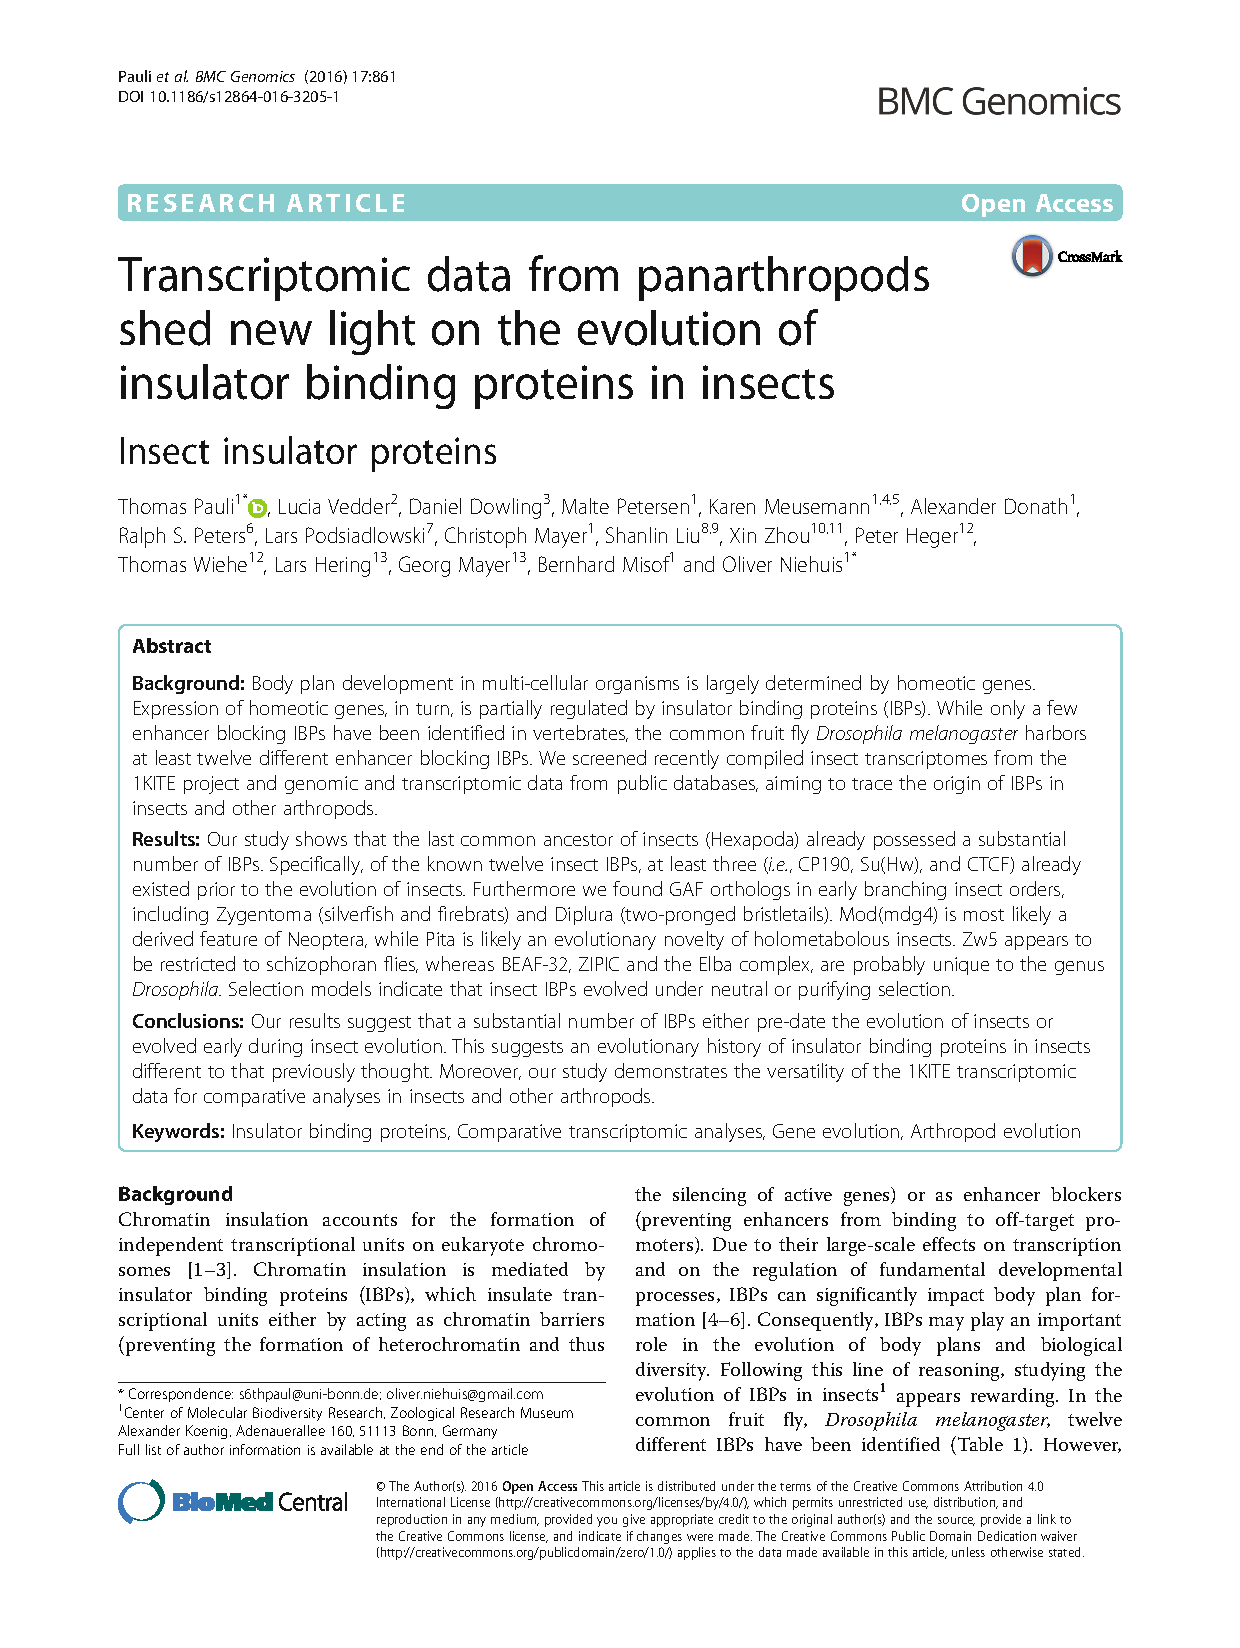
\includepdf[addtotoc={1,section,1,\citet{Pauli2016}: New insights on the evolution of insulator binding proteins in insects ,app:Pauli2016},pages=-]{appendix/A/Pauli2016}
\includepdf[addtotoc={1,section,1,\citet{Mayer2016}: BaitFisher: A software package for multispecies target DNA enrichment probe design ,app:Mayer2016},pages=-]{appendix/A/Mayer2016}
}

	%!TEX root = ../dissertation.tex
\chapter{Other co-authored publications}
\label{app:other-publications}

\ifdraft{%
	\section{\citet{Astrin2016}}
	\emptypages{24} % Astrin 2016
	\section{\citet{Kraaijeveld2016}}
	\emptypages{11} % Kraaijeveld2016
	\section{\citet{Struck2014}}
	\emptypages{17} % Struck2014
	\section{\citet{Peters2014}}
	\emptypages{16} % Peters2014
	\section{\citet{Misof2014}\label{app:Misof2014}}
	\emptypages{5} % Misof2014
	\section{\citet{Dell'Ampio2014}}
	\emptypages{11} % Dell'Ampio 2014
	\section{\citet{Niehuis2012}}
	\emptypages{5} % Niehuis2012
}%
{%
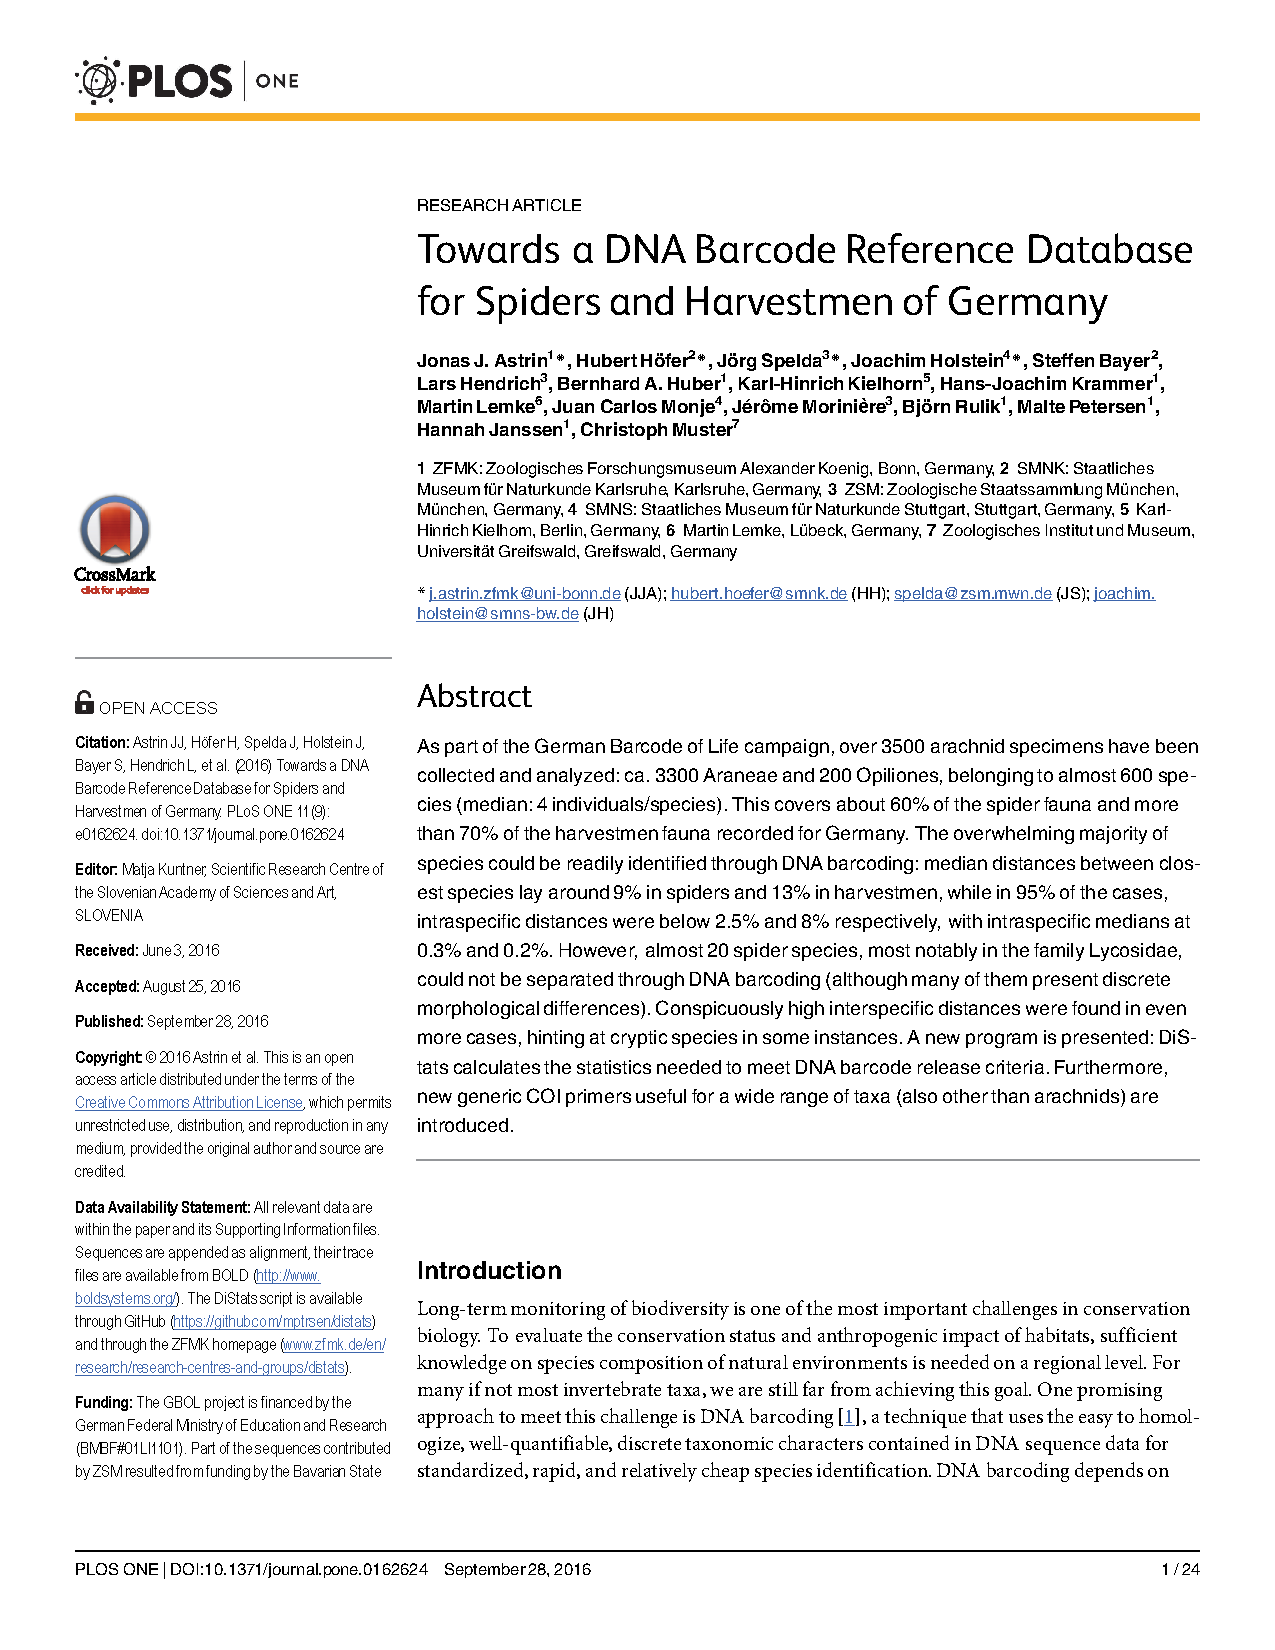
\includepdf[addtotoc={1,section,1,\citet{Astrin2016}: Towards a DNA barcode reference database for spiders and harvestmen of germany,app:Astrin2016},pages=-]{appendix/B/Astrin2016} % range without endpoints: from first to last
\includepdf[addtotoc={1,section,1,\citet{Kraaijeveld2016}: Decay of sexual trait genes in an asexual parasitoid wasp,app:Kraaijeveld2016},pages=-]{appendix/B/Kraaijeveld2016} % range without endpoints: from first to last
\includepdf[addtotoc={1,section,1,\citet{Struck2014}: Platyzoan paraphyly based on phylogenomic data supports a noncoelomate ancestry of Spiralia,app:Struck2014},pages=-]{appendix/B/Struck2014} % range without endpoints: from first to last
\includepdf[addtotoc={1,section,1,\citet{Peters2014}: The evolutionary history of holometabolous insects inferred from transcriptome-based phylogeny and comprehensive morphological data,app:Peters2014},pages=-]{appendix/B/Peters2014} % range without endpoints: from first to last
\label{app:Misof2014}
\includepdf[addtotoc={1,section,1,\citet{Misof2014}: Phylogenomics resolves the timing and pattern of insect evolution,app:Misof2014},pages=-]{appendix/B/Misof2014} % range without endpoints: from first to last
\includepdf[addtotoc={1,section,1,\citet{Dell'Ampio2014}: Decisive data sets in phylogenomics: lessons from studies on the phylogenetic relationships of primarily wingless insects,app:Dell'Ampio2014},pages=-]{appendix/B/DellAmpio2014} % range without endpoints: from first to last
\includepdf[addtotoc={1,section,1,\citet{Niehuis2012}: Genomic and morphological evidence converge to resolve the enigma of Strepsiptera,app:Niehuis2012},pages=-]{appendix/B/Niehuis2012} % range without endpoints: from first to last
}%

\end{appendices}

\backmatter

\end{document}
